 \documentclass{beamer}

\usepackage{amsthm,amssymb,amsmath}
\usepackage[round]{natbib}
\bibliographystyle{asa}
\usepackage{amsmath}
\usepackage{amsfonts}
\usepackage{amssymb}
\usepackage{amsthm}


\usepackage[normalem]{ulem}
\usepackage{booktabs}

\usepackage{calc,tikz,nicefrac}
\usetikzlibrary{positioning}
%\geometry{letterpaper}
%\usepackage{xcolor}
%\usepackage[usenames, dvipsnames]{color}

\def\mb{\mathbf}
\def\iid{\mathrm{i.i.d. }}
\def\bs{\boldsymbol}

\mode<presentation>
{
  \usetheme{metropolis}
%  \usetheme{Boadilla}
  %\usetheme{Warsaw}
  % or ...

  \setbeamercovered{transparent}
  % or whatever (possibly just delete it)
}

\def\mb{\mathbf}
\def\iid{\mathrm{i.i.d. }}
\def\bs{\boldsymbol}
\def\tbf{\textbf}
\def\t{^{\top}}
\def\bSig{\bs{\Sigma}}
\newcommand{\mcitet}[1]{\mbox{\citet{#1}}}
 

\usepackage[english]{babel}
\usepackage{verbatim}
% or whatever

\usepackage[latin1]{inputenc}
% or whatever
\usepackage{hyperref}

\usepackage{times}
\usepackage{color}
\usepackage[T1]{fontenc}

\newcommand{\Blue}{\color{blue}}
\newcommand{\ve}{\varepsilon}
\newcommand{\Perp}{\perp \! \! \! \perp}

\newtheorem{assumption}{Assumption}
\newtheorem{proposition}{Proposition}
\newtheorem{remark}{Remark}

\definecolor{forestgreen(web)}{rgb}{0.13, 0.55, 0.13}
\def\bcolor{\color{forestgreen(web)}}
%\def\bcolor{\color{green}}
\def\pcolor{\color{blue}}
\def\icolor{\color{magenta}}
\def\wcolor{\color{gray}}
\def\ycolor{\color{red}}
\newcommand{\argmax}{\operatornamewithlimits{arg\,max}}
\newcommand{\argmin}{\operatornamewithlimits{arg\,min}}
\def\inprobLOW{\rightarrow_p}
\def\inprobHIGH{\,{\buildrel p \over \rightarrow}\,}
\def\inprob{\,{\inprobHIGH}\,}
\def\indist{\,{\buildrel d \over \rightarrow}\,}
\def\F{\mathbb{F}}
\newcommand{\gmatrix}[1]{\begin{pmatrix} {#1}_{11} & \cdots &
    {#1}_{1n} \\ \vdots & \ddots & \vdots \\ {#1}_{m1} & \cdots &
    {#1}_{mn} \end{pmatrix}}
\newcommand{\iprod}[2]{\left\langle {#1} , {#2} \right\rangle}
\newcommand{\norm}[1]{\left\Vert {#1} \right\Vert}
\newcommand{\abs}[1]{\left\vert {#1} \right\vert}
\renewcommand{\det}{\mathrm{det}}
\newcommand{\rank}{\mathrm{rank}}
\newcommand{\spn}{\mathrm{span}}
\newcommand{\row}{\mathrm{Row}}
\newcommand{\col}{\mathrm{Col}}
\renewcommand{\dim}{\mathrm{dim}}
\newcommand{\prefeq}{\succeq}
\newcommand{\pref}{\succ}
\newcommand{\seq}[1]{\{{#1}_n \}_{n=1}^\infty }
\renewcommand{\to}{{\rightarrow}}
\providecommand{\Infected}{{\mathcal{I}}}
\providecommand{\Recovered}{{R}}

\providecommand{\Er}{{\mathrm{E}}}
\providecommand{\Var}{{\mathrm{Var}}}
\providecommand{\set}[1]{\left\{#1\right\}}
\providecommand{\plim}{\operatornamewithlimits{plim}}
\newcommand\indep{\protect\mathpalette{\protect\independenT}{\perp}}
\def\independenT#1#2{\mathrel{\setbox0\hbox{$#1#2$}%
    \copy0\kern-\wd0\mkern4mu\box0}}


\title[Impact of K-12 Schools and College Openings]
{The Impact of Opening K-12 Schools and Colleges on the Spread of COVID-19 in the U.S.}

%\subtitle
%{Include Only If Paper Has a Subtitle}
%\subtitle
%{A Celebration of Peter Phillips' Fourty Years at Yale Conference}


\author[Victor Chernozhukov, Hiroyuki Kasahara, Paul Schrimpf] % (optional, use only with lots of authors)
{Victor Chernozhukov\inst{1} \and Hiroyuki Kasahara\inst{2} \and Paul Schrimpf\inst{2}}
% - Give the names in the same order as the appear in the paper.
% - Use the \inst{?} command only if the authors have different
%   affiliation.

\institute[] % (optional, but mostly needed)
{
  \inst{1}%
  Department of Economics and Center for Statistics and Data Science, MIT
  \and
  \inst{2}%
  Vancouver School of Economics,
  UBC }



 
\date[January 2021] % (optional, should be abbreviation of conference name)
{}
% - Either use conference name or its abbreviation.
% - Not really informative to the audience, more for people (including
%   yourself) who are reading the slides online

\subject{}
% This is only inserted into the PDF information catalog. Can be left
% out.


% If you have a file called "university-logo-filename.xxx", where xxx
% is a graphic format that can be processed by latex or pdflatex,
% resp., then you can add a logo as follows:

% \pgfdeclareimage[height=0.5cm]{university-logo}{university-logo-filename}
% \logo{\pgfuseimage{university-logo}}



% Delete this, if you do not want the table of contents to pop up at
% the beginning of each subsection:
%\AtBeginSubsection[]
%{
%  \begin{frame}<beamer>
%    \frametitle{Outline}
%    \tableofcontents[currentsection,currentsubsection]
%  \end{frame}
%}


% If you wish to uncover everything in a step-wise fashion, uncomment
% the following command:

%\beamerdefaultoverlayspecification{<+->}


\begin{document}

\begin{frame}
  \titlepage
\end{frame}


 %----------------------------------------------------------------------------------------%

\begin{frame}
  \frametitle{Issue}%\vspace{-0.8cm}
\Large
  What is the impact of opening K-12 schools and colleges/universities on the spread of COVID-19 in the United States?
  
  
\end{frame}

%----------------------------------------------------------------------------------------%

 


 
%----------------------------------------------------------------------------------------%

\begin{frame}
  \frametitle{County-level Panel Data}\vspace{-0.05cm} 
  
  \begin{itemize}
  \item Data period: from May 1 to December 2.\medskip
  \item 3219 Counties \medskip
  \item {\ycolor Daily cases and deaths}: \underline{NYT}\medskip
 %  \item {\wcolor The number of tests}: Covid Tracking Project\medskip
  \item  {\pcolor  County-level policies}: mandatory masks, ban gathering more than 50, stay-at-home  \underline{\citep{killeen2020countylevel}}
 \medskip
   \item  {\pcolor  K-12 opening plans}: dates of K-12 school openings and the learning modes (in-person, hybrid, and remote) from \underline{EducationWeek}
 \medskip
 
\item {\pcolor  Foot trafic data}: visits to  colleges/universities, K-12 schools, restaurants, bars, gyms from \underline{SafeGraph}

%SafeGraph
%\item {\bcolor Behavior variables}:  ``Transit stations,''  ``Workplaces,''  ``Grocery \& pharmacy," and ``Retail \& recreation'' from Google Mobility Reports.  
  \end{itemize} 
  
We use  \underline{7 days moving averages} of all variables %  because of
%\begin{itemize}
%\item  idiosyncratic reporting delays,
%\item seasonality associated with the days of the week.
%\end{itemize}
%   

\end{frame}
 %----------------------------------------------------------------------------------------%

 %----------------------------------------------------------------------------------------% 
\begin{frame}{Evolutions of Cases and Visits to K-12 Schools and Colleges}
\begin{figure}[ht] 
%\caption{Evolution of Cases per 1000,  Case Growth, Visits to K-12 Schools, Colleges, Restaurants, Bars, Gyms, and Churches across U.S. counties \label{fig:evolution}}
\resizebox{0.8\columnwidth}{!}{
\begin{minipage}{\linewidth}
    \centering
        \begin{tabular}{cc} 
   (a) Case Growth &  (b)  Cases per 1000 \\
      \includegraphics[width=0.49\textwidth]{../tables_and_figures/nyt-dlogdc}&
      \includegraphics[width=0.49\textwidth]{../tables_and_figures/nyt-dcase_capita}\\ 
%   (b) Death Growth &  (c)  Deaths per 1000 \\
%      \includegraphics[width=0.49\textwidth]{tables_and_figures/nyt-dlogdd}&
%      \includegraphics[width=0.49\textwidth]{tables_and_figures/nyt-ddeath_capita}\\ 
  (c) Visits to K-12 Schools & (d) Visits to Colleges\\
  \includegraphics[width=0.49\textwidth]{../tables_and_figures/sg-school}&
  \includegraphics[width=0.49\textwidth]{../tables_and_figures/sg-college}\\
  (e) Visits to Restaurants & (f) Visits to Bars\\
  \includegraphics[width=0.49\textwidth]{../tables_and_figures/sg-restaurant}&
  \includegraphics[width=0.49\textwidth]{../tables_and_figures/sg-bar}\\
%  (h) Visits to Gyms & (i) Visits to Churches\\
%  \includegraphics[width=0.49\textwidth]{tables_and_figures/sg-gym}&
%  \includegraphics[width=0.49\textwidth]{tables_and_figures/sg-church}\\
    \end{tabular} 
  \end{minipage}}
\end{figure}

\end{frame}
 %----------------------------------------------------------------------------------------%

 %----------------------------------------------------------------------------------------% 
\begin{frame}
  \frametitle{Weekly Cases and Openings of K-12 Schools and Colleges} 
%  \begin{figure}
%  \centering
  
  \begin{figure}[ht]
%  \caption{Average daily cases are associated with different modes of opening K-12 schools and the per-device visits to K-12 schools and colleges/universities \label{fig:case-growth}} 
\resizebox{0.84\columnwidth}{!}{
\begin{minipage}{\linewidth}
    \centering
        \begin{tabular}{cc} 
    (a)  Cases by  K-12 opening modes & (b) K-12 visits by opening modes\\
    \hspace{-0.5cm}         \includegraphics[width=0.5\textwidth]{../tables_and_figures/schoolmode-weekcase-simple}&
   \hspace{-0.5cm}      \    \includegraphics[width=0.5\textwidth]{../tables_and_figures/schoolmode-weekvisits-simple}\\ 
  (c) Cases by K-12 school visits & (d)  Cases by college visits\\
   \hspace{-0.5cm}      \includegraphics[width=0.5\textwidth]{../tables_and_figures/school-weekcase-simple}&
  \hspace{-0.5cm}      \ \includegraphics[width=0.5\textwidth]{../tables_and_figures/college-weekcase-simple-2} % \\
%  (e) Cases by college visits&(f) Deaths by college visits\\
%  \includegraphics[width=0.49\textwidth]{tables_and_figures/college-weekcase-simple}&
%  \includegraphics[width=0.49\textwidth]{tables_and_figures/college-weekdeath-simple}
    \end{tabular} 
  \end{minipage}}
\end{figure}


%  \begin{minipage}{\textwidth}
%    \centering
%    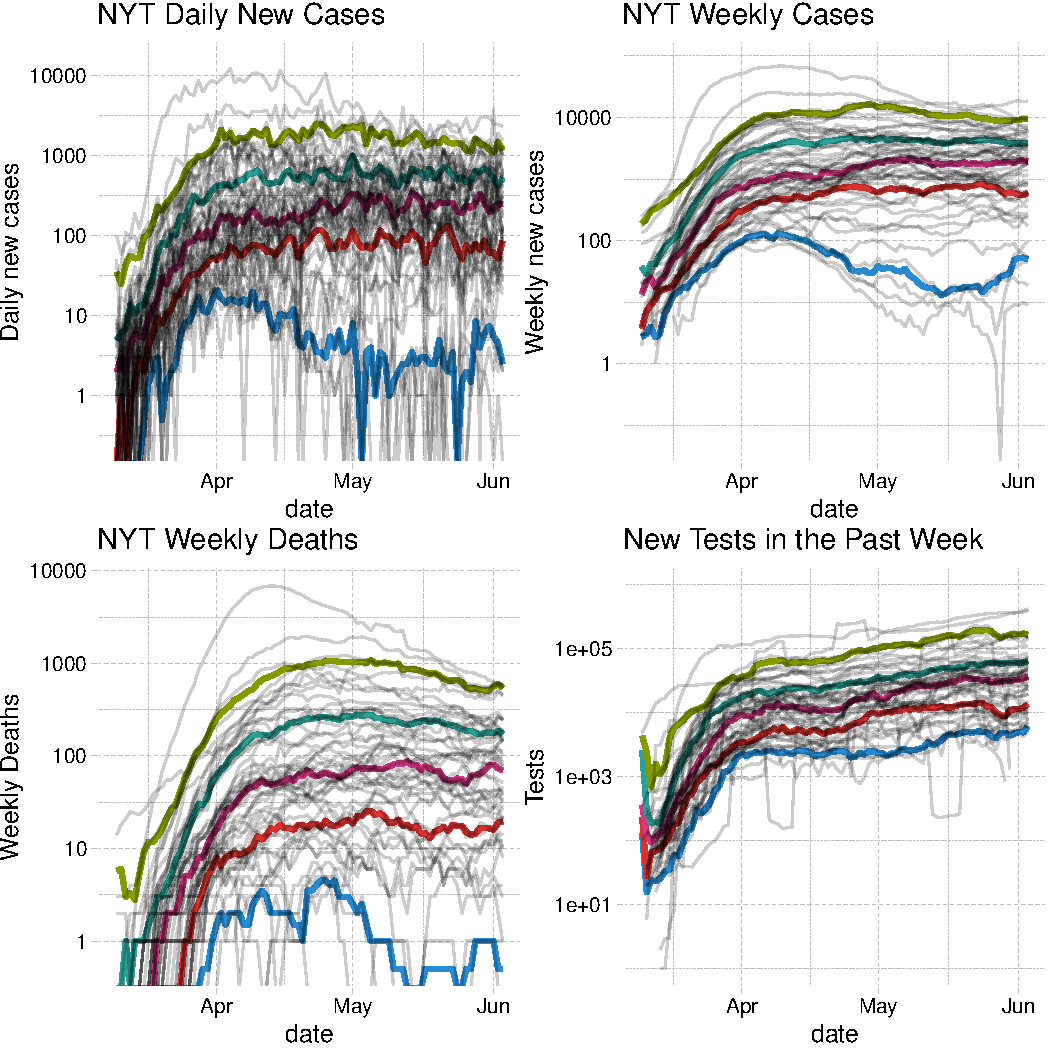
\includegraphics[width=0.8\textwidth,height=0.65\textwidth]{tables_and_figures/casesdeaths_q}
%%      \footnotetext{Thin gray lines are case or death growth in each
%%      state and date. Thicker colored lines are quantiles of case or
%%      death growth conditional on date.}
%  \end{minipage}
%     \begin{flushleft}
%      \footnotesize Thin gray lines are the log of cases, death, and tests  in each
%      state and date. Thicker colored lines are their quantiles conditional on date.
%      \end{flushleft}
%\end{figure}

\end{frame} 
%----------------------------------------------------------------------------------------%



 %----------------------------------------------------------------------------------------% 
\begin{frame}
  \frametitle{Dane County, Wisconsin} 


\begin{figure}[ht]
%  \caption{The number of cases by age groups and the number of visits to K-12 schools, colleges/universities, and bars in Dane county, WI \label{fig:dane}} 
\centering
   \begin{minipage}{0.6\linewidth}
 \hspace{-0.5cm}      \includegraphics[width=1.25\textwidth]{../tables_and_figures/dane.jpeg}
       \end{minipage}
\end{figure} 

\end{frame} 
%----------------------------------------------------------------------------------------%



 %----------------------------------------------------------------------------------------% 
\begin{frame}
  \frametitle{County-level Panel Data Regression} 
\begin{table}[!htbp] \centering
% \caption{The Effect of School/College Openings and NPI Policies on Case Growth in the United States: Cross-County Panel Regressions}\vspace{-0.3cm}
 \label{tab:PItoY} 
\resizebox{0.65\columnwidth}{!}{
\begin{tabular}{@{\extracolsep{1pt}}lcccc} 
\\[-1.8ex]\hline 
\hline \\[-1.8ex] 
 & \multicolumn{4}{c}{\textit{Dependent variable: Weekly Case Growth Rates}} \\ 
\cline{2-5} 
 % & \multicolumn{4}{c}{$\Delta \log \Delta C_{it}$} \\ 
%\\[-1.8ex] & (1) & (2) & (3) & (4)\\ 
\hline \\[-1.8ex] 
 {\pcolor College Visits}, 14 days lag &{\pcolor  0.190}$^{***}$ & {\pcolor 0.462}$^{***}$ & {\pcolor 0.173}$^{***}$ &{\pcolor  0.337}$^{**}$ \\ 
  & (0.064) & (0.151) & (0.065) & (0.159) \\ 
   {\ycolor K-12 Visits}, 14 days lag & {\ycolor 0.671}$^{***}$ &  & {\ycolor 0.509}$^{***}$ &  \\ 
  & (0.070) &  & (0.067) &  \\ 
 {\bcolor K-12 Open Full}, 14 days lag  &  & {\bcolor 0.143}$^{***}$ &  & {\bcolor 0.100}$^{***}$ \\ 
  &  & (0.023) &  & (0.026) \\ 
  {\bcolor K-12 Open Hybrid}, 14 days lag &  & {\bcolor 0.095}$^{***}$ &  &{\bcolor  0.050}$^{**}$ \\ 
  &  & (0.021) &  & (0.025) \\ 
 {\bcolor K-12 Open Remote}, 14 days lag &  &{\bcolor  0.032} &  & {\bcolor $-$0.005} \\ 
  &  & (0.021) &  & (0.024) \\ \hline
Mask Mandates, 14 days lag & $-$0.079$^{***}$ & $-$0.060$^{***}$ & $-$0.089$^{***}$ & $-$0.036$^{**}$ \\ 
  & (0.011) & (0.015) & (0.010) & (0.015) \\ 
 Ban Gatherings, 14 days lag   & $-$0.241$^{***}$ & $-$0.208$^{***}$ & $-$0.088$^{**}$ & $-$0.130$^{*}$ \\ 
  & (0.029) & (0.052) & (0.042) & (0.074) \\ 
 Stay at Home, 14 days lag & $-$0.194$^{***}$ & $-$0.150$^{***}$ & $-$0.061 & $-$0.065 \\ 
  & (0.031) & (0.049) & (0.042) & (0.066) \\ \hline 
 log(Cases), 14 days lag & $-$0.109$^{***}$ & $-$0.122$^{***}$ & $-$0.104$^{***}$ & $-$0.107$^{***}$ \\ 
  & (0.004) & (0.009) & (0.005) & (0.010) \\ 
 log(Cases), 21 days lag  & $-$0.048$^{***}$ & $-$0.024$^{*}$ & $-$0.054$^{***}$ & $-$0.034$^{***}$ \\ 
  & (0.005) & (0.012) & (0.005) & (0.012) \\ 
 log(Cases), 28 days lag   & $-$0.029$^{***}$ & $-$0.058$^{***}$ & $-$0.029$^{***}$ & $-$0.052$^{***}$ \\ 
  & (0.004) & (0.010) & (0.004) & (0.009) \\  
   \hline \hline
\alert{County FE} & Yes & Yes &  Yes  &  Yes  \\  
\alert{State$\times$ Month FE}& Yes & Yes &  No  &  No  \\ 
\alert{State$\times$ Week FE}&No & No &  Yes  &  Yes  \\ 
\hline \\[-1.8ex] 
Observations & 586,902 & 131,890 & 586,902 & 131,890 \\ 
%R$^{2}$ & 0.055 & 0.086 & 0.098 & 0.203 \\ 
\hline 
\hline \\[-1.8ex] 
\textit{Note:}  & \multicolumn{4}{r}{$^{*}$p$<$0.1; $^{**}$p$<$0.05; $^{***}$p$<$0.01}  
\end{tabular}} 
\end{table}

\end{frame} 
%----------------------------------------------------------------------------------------%


 %----------------------------------------------------------------------------------------% 
\begin{frame}
  \frametitle{Sensitivity Analysis} 


\begin{flushleft}
\begin{figure}[ht]
 % \caption{Sensitivity analysis for the estimated coefficients of K-12 visits and college visits of case and death growth regressions \label{fig:sensitivity}}  
     \begin{tabular}{cc}  
        (a) Case Growth Regression & (b) Death Growth Regression \\
    \hspace{-0.5cm}   \includegraphics[width=0.5\textwidth]{../tables_and_figures/school-college-whisker-cases.pdf} 
        &
       \includegraphics[width=0.5\textwidth]{../tables_and_figures/school-college-whisker-deaths.pdf} 
       \end{tabular}
       
\end{figure} 
\end{flushleft}

\end{frame} 
%----------------------------------------------------------------------------------------%


 %----------------------------------------------------------------------------------------% 
\begin{frame}
  \frametitle{Visits to colleges and K-12 schools and visits to restaurants, bars, gyms, and churches.} 

\begin{table}[!htbp] \centering
% \caption{The Effect of School/College Openings and NPI Policies on Mobility in the United States: Cross-County Panel Regressions}\vspace{-0.3cm}
 \label{tab:PItoY} 
\resizebox{0.65\columnwidth}{!}{
 \begin{tabular}{@{\extracolsep{1pt}}lcccc} 
\\[-1.8ex]\hline 
\hline \\[-1.8ex] 
 & \multicolumn{4}{c}{\textit{Dependent variable:}} \\ 
\cline{2-5} 
 & {\ycolor Restaurant Visits} &  {\ycolor Bar Visits}  & {\ycolor Gym Visits} & {\ycolor Church  Visits} \\ 
\\[-1.8ex] & (1) & (2) & (3) & (4)\\ 
\hline \\[-1.8ex] 
  {\pcolor College Visits }&{\pcolor  0.392}$^{***}$ &{\pcolor  0.026}$^{***}$ &{\pcolor  0.023}$^{**}$ &{\pcolor  0.036}$^{***}$ \\ 
  & (0.091) & (0.007) & (0.009) & (0.005) \\ 
{\pcolor   K-12 School Visits} &{\pcolor  0.324}$^{***}$ &{\pcolor  0.044}$^{***}$ &{\pcolor  0.028}$^{***}$ &{\pcolor  0.053}$^{***}$ \\ 
  & (0.044) & (0.016) & (0.006) & (0.013) \\ \hline
   
Mandatory mask & 0.287 & 0.112$^{***}$ & 0.091$^{***}$ & 0.102$^{***}$ \\ 
  & (0.299) & (0.041) & (0.033) & (0.031) \\ 
  Ban gatherings  & $-$0.773$^{***}$ & $-$0.122$^{***}$ & $-$0.326$^{***}$ & $-$0.018 \\ 
  & (0.143) & (0.017) & (0.029) & (0.021) \\ 
  Stay at home & $-$1.348$^{***}$ & $-$0.239$^{***}$ & $-$0.317$^{***}$ & $-$0.010 \\ 
  & (0.156) & (0.027) & (0.026) & (0.017) \\ \hline
  
  log(Cases) & $-$0.021 & 0.001 & $-$0.009$^{**}$ & $-$0.016$^{***}$ \\ 
  & (0.026) & (0.004) & (0.004) & (0.003) \\ 
 log(Cases), 7 days lag & $-$0.045$^{**}$ & $-$0.001 & $-$0.015$^{***}$ & $-$0.017$^{***}$ \\ 
  & (0.019) & (0.004) & (0.003) & (0.003) \\ 
 log(Cases), 14 days lag & $-$0.171$^{***}$ & $-$0.014$^{***}$ & $-$0.022$^{***}$ & $-$0.008$^{**}$ \\ 
  & (0.026) & (0.004) & (0.004) & (0.003) \\  
  \hline \hline
\alert{County FE} & Yes & Yes &  Yes  &  Yes  \\   
\alert{State$\times$ Week FE}&Yes  &  Yes  &  Yes  &  Yes  \\ 
%State$\times$ Week FE&Yes  &  Yes  &  Yes  &  Yes  \\ 
\hline \\[-1.8ex] 
Observations & 586,904 & 586,904 & 586,904 & 586,904 \\ 
R$^{2}$ & 0.883 & 0.797 & 0.859 & 0.846 \\ 
\hline 
\hline \\[-1.8ex] 
\textit{Note:}  & \multicolumn{4}{r}{$^{*}$p$<$0.1; $^{**}$p$<$0.05; $^{***}$p$<$0.01} \\ 
\end{tabular} 
}
\end{table}
 
\end{frame} 
%----------------------------------------------------------------------------------------%



\begin{frame}[allowframebreaks]
\frametitle{Bibliography}
%\large
\footnotesize
\bibliography{../covid}
\end{frame}

\begin{frame}{Correlation matrix}


\begin{figure}[ht] 
%\caption{Correlation across variables \label{fig:corr}}
 
\begin{flushleft}
\resizebox{0.6\columnwidth}{!}{
\begin{minipage}{\linewidth} 
\begin{tabular}{lcccccccccccc}
\toprule
\rotatebox{90}{ } & \rotatebox{90}{Restaurant Visits} & \rotatebox{90}{Bar Visits} & \rotatebox{90}{Gym Vists} & \rotatebox{90}{Church Vists} & \rotatebox{90}{Mandatory mask} & \rotatebox{90}{Ban gatherings >50} & \rotatebox{90}{Stay at home} & \rotatebox{90}{College Visits} & \rotatebox{90}{K-12 Visits} & \rotatebox{90}{Open K-12 full} & \rotatebox{90}{Open K-12 hybrid} & \rotatebox{90}{Open K-12 remote}\\
\midrule
Restaurant Visits & 1.00 &  &  &  &  &  &  &  &  &  &  & \\
Bar Visits & 0.21 & 1.00 &  &  &  &  &  &  &  &  &  & \\
Gym Vists & 0.51 & 0.19 & 1.00 &  &  &  &  &  &  &  &  & \\
Church Vists & 0.13 & 0.04 & -0.02 & 1.00 &  &  &  &  &  &  &  & \\
Mandatory mask & 0.14 & 0.01 & 0.18 & -0.07 & 1.00 &  &  &  &  &  &  & \\
\addlinespace
Ban gatherings >50 & 0.17 & -0.03 & 0.07 & -0.00 & -0.04 & 1.00 &  &  &  &  &  & \\
Stay at home & -0.00 & -0.04 & -0.03 & -0.08 & -0.09 & 0.14 & 1.00 &  &  &  &  & \\
College Visits & 0.21 & 0.06 & 0.18 & 0.08 & 0.09 & -0.02 & -0.04 & 1.00 &  &  &  & \\
K-12 Visits & -0.02 & 0.05 & -0.02 & 0.30 & 0.07 & -0.11 & -0.18 & 0.09 & 1.00 &  &  & \\
Open K-12 full & -0.01 & -0.06 & -0.07 & 0.25 & -0.06 & -0.08 & -0.13 & 0.10 & 0.53 & 1.00 &  & \\
\addlinespace
Open K-12 hybrid & -0.05 & 0.04 & 0.04 & 0.05 & 0.13 & -0.10 & -0.09 & 0.09 & 0.29 & -0.15 & 1.00 & \\
Open K-12 remote & 0.06 & 0.07 & 0.19 & -0.05 & 0.32 & 0.00 & -0.14 & 0.06 & 0.05 & -0.19 & -0.14 & 1.00\\
\bottomrule
\end{tabular}  
 \end{minipage}}
 
\end{flushleft}
\end{figure}

\end{frame}

\end{document}

%\begin{frame}
%  \frametitle{Literature}%\vspace{-0.8cm}
% 
% \footnotesize
%\begin{itemize}
%
%\item The impact of non
%pharmaceutical interventions on Covid-19  cases:  \cite{hsiang2020},  \cite{courtemanche2020},  \cite{avery2020} for review.
%
% 
%\item The impact of social distancing policies on behavior in the US is mixed:  \cite{abouk2020}, \cite{maloney2020},  \cite{gupta2020}, \cite{anderson2020} 
%
%\item \cite{pei2020}  provides simulation of implementing all policies 1-2 weeks earlier.  
%
%\item Model simulations by epidemiologists  \citep[e.g.,][]{ferguson2020}. Substantial uncertainty in parameters  \citep{avery2020,
% stock2020}
% 
% \item  \cite{NBERw27128} estimate a SIRD model that captures feedback from daily deaths
%to future behavior and infections.
%
%\item No existing experimental evidence for face mask. Our work is complementary to the medical observational evidence reviewed in  \cite{Greenhalghm2020} and \cite{howard2020}, the laboratory findings of \cite{hou2020}, as well as the findings in  \cite{abaluck2020}, \cite{Mitze2020}, and \cite{miyazawa2020}.
%  
%\end{itemize}
%
%\end{frame}
%
%%----------------------------------------------------------------------------------------%

 

 


% %----------------------------------------------------------------------------------------%
%
%\begin{frame}
%  \frametitle{Contributions of this paper}\vspace{-0.05cm}
% 
% \begin{enumerate}
% \item The causal framework on how the Covid-19 spread  is dynamically determined by policies and human behavior.  \smallskip
% \begin{itemize}
% \item Direct  vs. indirect effect of policies.
% \item People voluntarily adjust their behavior in response to new information on reported cases/deaths.
% \item Dynamic feedback. \smallskip
% \end{itemize}
% \item Regression analysis on how the growth rates of  Covid-19 cases/deaths are determined by policies and behavior using the US state-level data.  \smallskip
% \item Counterfactual experiments \smallskip
% \begin{itemize}
% \item What if mandatory face mask policy had been adopted everywhere on March 14th? \smallskip
% \item What if no stay-at-home (shelter-in-place) orders?
%%\item What if no closure of non-essential businesses?
% \end{itemize}
% \end{enumerate}
%
%\end{frame}
%
%%----------------------------------------------------------------------------------------%

 


 %----------------------------------------------------------------------------------------%

\begin{frame}
  \frametitle{Causal Model}\vspace{-0.05cm}
 

\footnotesize
\begin{figure}[ht]
\begin{center}
\begin {tikzpicture}[-latex, auto, node distance =1.5cm and 3cm, on grid, thick,
  empty/.style ={circle, top color=white, bottom color = white, draw, white, text=white , minimum width =1.25 cm},
  policy/.style ={circle, top color=white, bottom color = blue, draw, black, text=black , minimum width =1.25 cm},
    behavior/.style ={circle, top color=white, bottom color = green, draw, black, text=black , minimum width =1.25 cm},
  observed/.style ={circle, top color=white, bottom color = magenta, draw, black, text=black , minimum width =1.25 cm} ,
   confounder/.style ={circle, top color=white, bottom color =  gray, draw, black, text=black , minimum width =1.25 cm} ,
outcome/.style ={circle, top color=white, bottom color = red, draw, black, text=black , minimum width =1.25 cm} ]

\node[policy]   (P) {\tiny $P_{it}$};
\node[empty] (E) [below=of P] {\tiny $I_{it}$};
\node[outcome]  (Y)[ right =of E] {\tiny $Y_{it+\ell}$};
\node[behavior] (B) [below =of E] {\tiny $B_{it}$};
\node[observed] (I) [left =of P] {\tiny $I_{it}$};
\node[confounder] (W) [left=of B] {\tiny  $W_{it}$};
\path[->] (P) edge (Y);
\path[->] (B) edge (Y);
\path[->] (P) edge (B);
\path[->] (I) edge (B);
\path[->] (I) edge (P);
\path[->] (W) edge (Y);
\path[->] (W) edge (B);
\path[->] (W) edge (P);
\path[->] (W) edge (I);
\path[->] (I) edge (Y);

\end{tikzpicture} \end{center}
%\caption{P. Wright type causal path diagram for our model. }\label{Wright}
\end{figure}
\small
\begin{itemize}
\item ${\ycolor  Y_{it+\ell}}$: the \textit{forward}  growth rate of cases/deaths
\item ${\pcolor  P_{it}}$: the lagged policies (e.g., mandatory face mask policy)
\item ${\bcolor  B_{it}}$: the lagged behavior variables (Google mobility measures)
 
\item ${\icolor  I_{it}}$: information on transmission risks (past cases and deaths) 
 
\item ${\wcolor  W_{it}}$: confounders (state-level characteristics, month dummies)
\end{itemize}


\end{frame}

%----------------------------------------------------------------------------------------%

\begin{frame}
 
  \frametitle{Structural Equation Model   and Orthogonality Restrictions}\vspace{-0.05cm}
 

	\begin{align}
   &  {\ycolor  Y_{it+\ell}}
    = {\bcolor\alpha ' B_{it}} + {\pcolor\pi 'P_{it}} + {\icolor\mu'I_{it}} + {\wcolor\delta_Y 'W_{it}}  + \varepsilon^y_{it},
    &  & \varepsilon^y_{it} \perp {\bcolor B_{it}}, {\pcolor P_{it}}, {\icolor I_{it}}, {\wcolor W_{it}} \label{eq:R1} \tag{BPI$\to$Y} \\
    &  {\bcolor B_{it}}
     =  {\pcolor \beta' P_{it}} + {\icolor \gamma'I_{it}} +  {\wcolor \delta_B' W_{it}} + \varepsilon^b_{it},
   & & \varepsilon^b_{it} \perp {\pcolor P_{it}}, {\icolor I_{it}}, {\wcolor W_{it}}  \label{eq:R2} \tag{PI$\to$B} % \\
%    & {\pcolor P_{it}}
%    =  {\icolor\eta'I_{it}} + {\wcolor \delta_P' W_{it}} +   \varepsilon^p_{it},   & & \varepsilon^p_{it} \perp   {\icolor I_{it}}, {\wcolor W_{it}} \label{eq:R3}  \tag{I$\to$P}
       \end{align}
and
\begin{align}
   {\ycolor  Y_{it+\ell}} 
   = ( {\pcolor\pi'}+ {\bcolor\alpha '}  {\pcolor \beta' }  )
    {\pcolor P_{it}} +(  {\icolor  \mu'}+{\bcolor\alpha '}  {\icolor \gamma'})
    {\icolor I_{it} }+ {\wcolor \bar \delta 'W_{it}}  + \bar \varepsilon_{it},  \quad  &  \bar \varepsilon_{it} \perp
  {\pcolor P_{it}},  {\icolor I_{it}}, {\wcolor W_{it}}.  \label{eq:R4} \tag{PI$\to$Y}
\end{align} 
\begin{itemize}
\item ${\pcolor\pi'}$:\quad\   \underline{direct} effect of policy. \smallskip
\item  ${\bcolor\alpha '}  {\pcolor \beta' }$:\   \underline{indirect} effect of policy on infection through behavior.\smallskip
\end{itemize}
%\begin{itemize}
%%\item (\ref{eq:R1}) and (\ref{eq:R2}) imply (\ref{eq:R4}). 
%% \item The system is over-identified. %:  $E[\epsilon^y {\bcolor B_{it}}]=0$.
% 
%\end{itemize}


\end{frame}

%----------------------------------------------------------------------------------------%



%----------------------------------------------------------------------------------------%

\begin{frame}
  \frametitle{Dynamic feedback }
  
\begin{figure}[ht]
\begin{center}
\begin {tikzpicture}[-latex, auto, node distance =3cm and 3cm, on grid, thick,
  empty/.style ={circle, top color=white, bottom color = white, draw, white, text=white , minimum width =1.25 cm},
  policy/.style ={circle, top color=white, bottom color = blue, draw, black, text=black , minimum width =1.25 cm},
    behavior/.style ={circle, top color=white, bottom color = ForestGreen, draw, black, text=black , minimum width =1.25 cm},
  observed/.style ={circle, top color=white, bottom color = magenta, draw, black, text=black , minimum width =1.25 cm} ,
   confounder/.style ={circle, top color=white, bottom color =  gray, draw, black, text=black , minimum width =1.25 cm} ,
outcome/.style ={circle, top color=white, bottom color = red, draw, black, text=black , minimum width =1.25 cm},
myarrow/.style={-Stealth}]

\node[observed] (I)  {\tiny $I_{i,t-\ell}$};
\node[outcome]  (Y)[below=of I ]{\tiny $Y_{it}$};
\node[observed] (In)  [right=of I ]{\tiny $I_{it}$};
\node[outcome]  (Yn)[below=of In ]{\tiny $Y_{i,t+\ell}$};
\node[observed] (Inn)  [right=of In ]{\tiny $I_{i,t+\ell}$};
\node[outcome]  (Ynn)[below=of Inn ]{\tiny $Y_{i,t+2\ell}$};
 \draw [->] (I) -- node[sloped,font=\small,below] {\tiny SEM(t-$\ell$)} (Y);
 \draw [->] (I) --  (In);
 \draw [->] (In) -- node[sloped,font=\small,below] {\tiny SEM(t)} (Yn);
\draw [->] (Y) --  (In);
\draw [->] (In) --  (Inn);
 \draw [->] (Inn) -- node[sloped,font=\small,below] {\tiny SEM(t+$\ell$) } (Ynn);
\draw [->] (Yn) --  (Inn);
\end{tikzpicture} \end{center}
%\caption{ Dynamic System Induced by Information Structure and SEM}\label{fig:DynS}
\end{figure}  
 $$
{\icolor I_{it}} = \left ( {\ycolor Y_{it}},  \sum_{m=0}^{t/\ell}
{\ycolor Y_{i,t - \ell m}} \right) ' =\left (  \text{lagged case growth}, \text{lagged cases} \right)
 $$
 
 
 



\end{frame}

%----------------------------------------------------------------------------------------%

%----------------------------------------------------------------------------------------%

\begin{frame}
  \frametitle{Susceptible-Infectious-Recovered (SIR)  Model with testing}\vspace{-0.05cm}
   
 SIR Model with confirmed cases $ \dot{C}(t)$ and testing $\tau(t)$:\bigskip
\begin{align*}
  \dot{S}(t)  = -\frac{S(t)}{N} \beta(t) \Infected(t),\qquad 
 & \dot{\Infected}(t)   = \frac{S(t)}{N} \beta(t) \Infected(t) - \gamma  \Infected(t), 
 \end{align*}
 \begin{align*}
  % \frac{S(t-\ell)}{N} \beta(t-\ell)  \Infected(t-\ell) \label{eq:i} \\
  \dot{\Recovered}(t)   = (1-\kappa) \gamma  \Infected(t),\qquad %  \frac{S(t-\ell)}{N} \beta(t-\ell)    \Infected(t-\ell) \label{eq:r} \\
 &  \dot{D}(t) = \kappa \gamma \Infected(t), %  \frac{S(t-\ell)}{N} \beta(t-\ell)   \Infected(t-\ell)
\qquad \dot{C}(t) = \tau(t) \Infected(t). \qquad
\end{align*}\smallskip
 
  
  Differentiating  { $\dot{C}(t) = \tau(t) \Infected(t)$} and $ \dot{D}(t) = \kappa \gamma \Infected(t)$,\bigskip
  \begin{align*}
    \frac{\ddot{C}(t)}{\dot{C}(t)}
              & =
                \frac{S(t)}{N} \beta(t) -\gamma  + \frac{\dot{\tau}(t)}{\tau(t)},
                \end{align*} 
                  \begin{align*}
    \frac{\ddot{D}(t)}{\dot{D}(t)}
              & =
                \frac{S(t)}{N} \beta(t) -\gamma.
                \end{align*}
                
                
 
 
%\draw [->] (Yn) --  (Inn);
%\end{tikzpicture} \end{center}
%%\caption{ Dynamic System Induced by Information Structure and SEM}\label{fig:DynS}
%\end{figure}
% $$
%{\icolor I_{it}} = \left ( {\ycolor Y_{i,t-\ell}},  \sum_{m=1}^{t/\ell}
%{\ycolor Y_{i,t - \ell m}} \right)  =\left (  \text{lagged case growth}, \text{lagged cases} \right)
% $$


 
\end{frame}

%----------------------------------------------------------------------------------------%


%----------------------------------------------------------------------------------------%

\begin{frame}
  \frametitle{SIR Model and Empirical Specification}\vspace{-0.05cm}
   
       Discrete-time analogue  with $\frac{S(t)}{N} \approx 1$ and\\ \smallskip
       $$\underbrace{ \beta(t) }_{\text{infection rate}} \approx   X_{i,t-{\Blue \ell}}'  \theta + \epsilon_{it}$$    \\ \smallskip
       with\smallskip
$$
X_{it} = \text{policy and behavior variables}
$$ \\\smallskip
%       where
%$
%X_{i,t-{\Blue \ell}}  = \text{policy and behavior variables}
%$\\ \medskip
$\Rightarrow$\medskip   
   \begin{align*}            
\underbrace{ {\ycolor \Delta \log \Delta C_{it}} }_{\text{growth rate of cases}}&   =  X_{i,t-{\Blue 14}}' \theta + \epsilon_{it} - \gamma+\delta_T \underbrace{ {\wcolor \Delta
      \log(T)_{it}}}_{\text{growth rate of tests}}\\
      &\quad \\
\underbrace{ {\ycolor \Delta \log \Delta D_{it}}  }_{\text{growth rate of deaths}}  & = X_{i,t-{\Blue 21}}' \theta + \epsilon_{it} - \gamma\smallskip 
                 \end{align*}      

\end{frame}

%----------------------------------------------------------------------------------------%


 
%----------------------------------------------------------------------------------------%

\begin{frame}
  \frametitle{Data}\vspace{-0.05cm} 
  
  \begin{itemize}
  \item Data Period: from March 7 to June 3.\medskip
  \item {\ycolor Daily cases and deaths}: NYT, JHU, Covid Tracking Project.\medskip
  \item {\wcolor The number of tests}: Covid Tracking Project\medskip
  \item  {\pcolor US state policies}:
\cite{raifman2020}.\medskip
\item {\bcolor Behavior variables}:  ``Transit stations,''  ``Workplaces,''  ``Grocery \& pharmacy," and ``Retail \& recreation'' from Google Mobility Reports.  
  \end{itemize} 
  
We use  \underline{7 days moving averages} of all variables %  because of
%\begin{itemize}
%\item  idiosyncratic reporting delays,
%\item seasonality associated with the days of the week.
%\end{itemize}
%   

\end{frame}
%----------------------------------------------------------------------------------------%
 

 %----------------------------------------------------------------------------------------%

\begin{frame}
  \frametitle{Daily/Weekly Cases,  Weekly Deaths, and Weekly Tests} 
  \begin{figure}
  \centering
  \begin{minipage}{\textwidth}
    \centering
    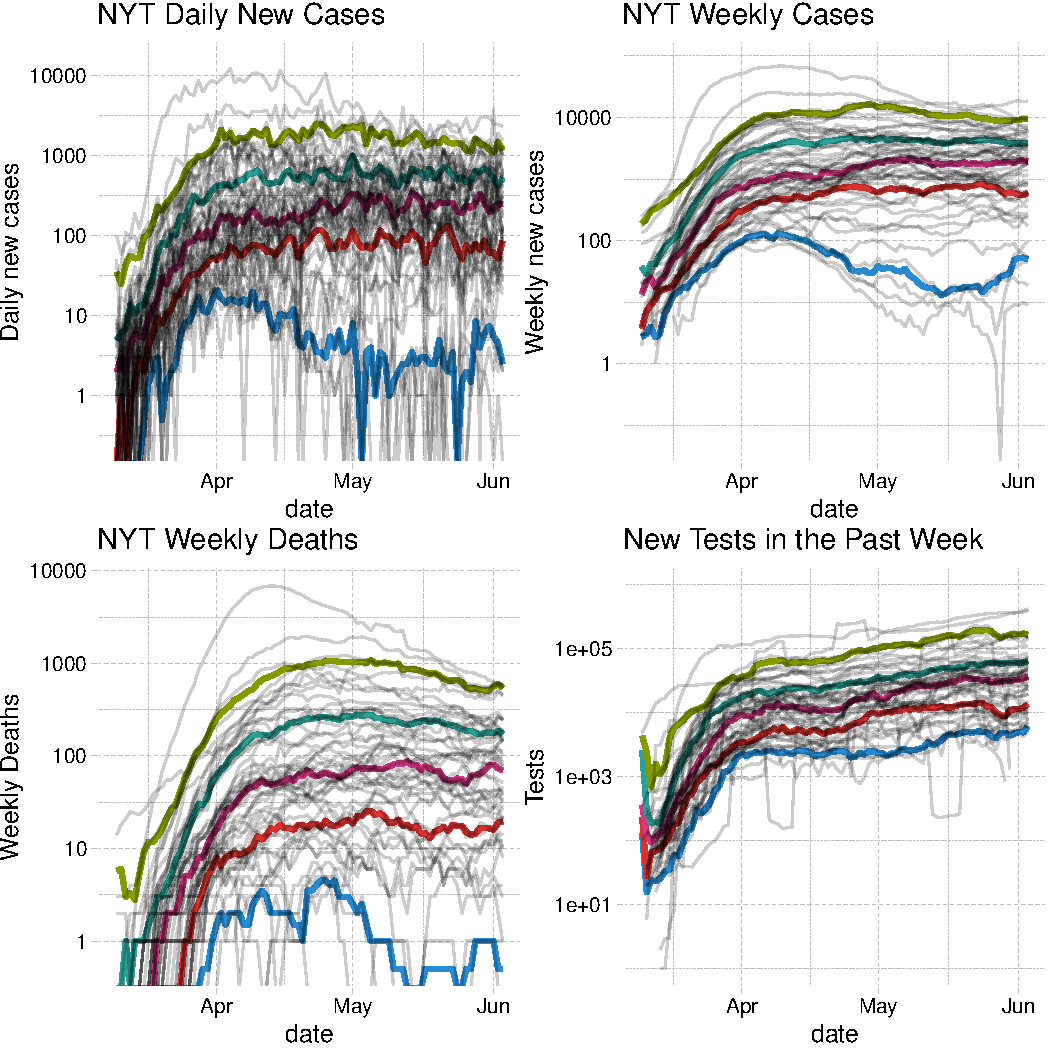
\includegraphics[width=0.8\textwidth,height=0.65\textwidth]{tables_and_figures/casesdeaths_q}
%      \footnotetext{Thin gray lines are case or death growth in each
%      state and date. Thicker colored lines are quantiles of case or
%      death growth conditional on date.}
  \end{minipage}
     \begin{flushleft}
      \footnotesize Thin gray lines are the log of cases, death, and tests  in each
      state and date. Thicker colored lines are their quantiles conditional on date.
      \end{flushleft}
\end{figure}

\end{frame}

%----------------------------------------------------------------------------------------%

%----------------------------------------------------------------------------------------%

\begin{frame}
  \frametitle{The Evolution of  ``Transit stations'' and ``Workplaces''}\vspace{-0.2cm}
\begin{figure} %\caption{The Evolution of  Transit stations and Workplaces\label{fig:transit-workplaces}}\vspace{0.1cm}
  \begin{minipage}{\linewidth}
    \begin{tabular}{c}
    \textbf{Transit}\\
      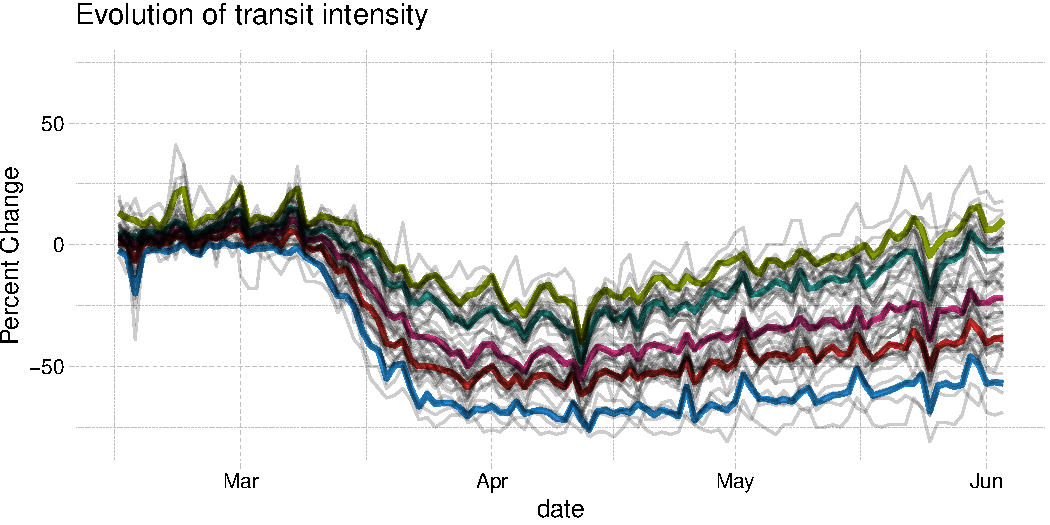
\includegraphics[width=0.6\linewidth]{../tables_and_figures/transit}\\ 
      \textbf{Workplaces}\\
      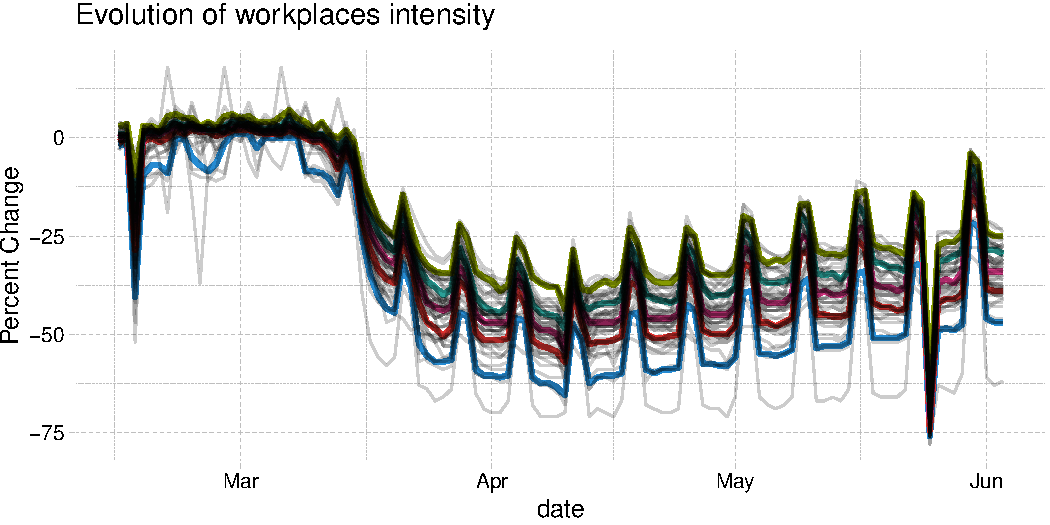
\includegraphics[width=0.6\linewidth]{../tables_and_figures/workplaces}
       \end{tabular}
       \end{minipage}
        \begin{flushleft}
%        \scriptsize{This figure shows the evolution of ``Transit stations'' and  ``Workplaces'' of Google Mobility
%      Reports. Thin gray lines are the value in each state and date. Thicker colored lines are
%      quantiles of the variables conditional on date.}
      \end{flushleft}
\end{figure}
   
\end{frame}
%----------------------------------------------------------------------------------------% 



%----------------------------------------------------------------------------------------%

\begin{frame}
  \frametitle{Portion of states with each
    policy}\vspace{-0.05cm}

\begin{figure}[ht]%\caption{Portion of states with each   policy \label{fig:policyportion}}
  \begin{minipage}{1.3\linewidth}
    \begin{tabular}{ccc}
      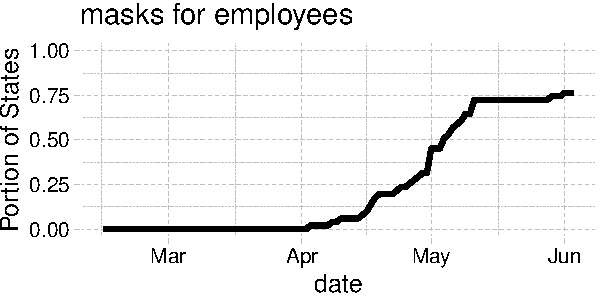
\includegraphics[width=0.33\textwidth]{pmaskbus_p}
      & \quad&
        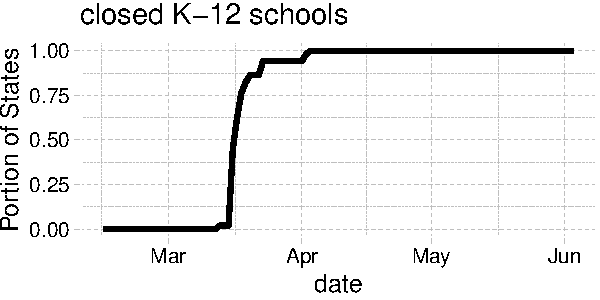
\includegraphics[width=0.33\textwidth]{pk12_p}\\
        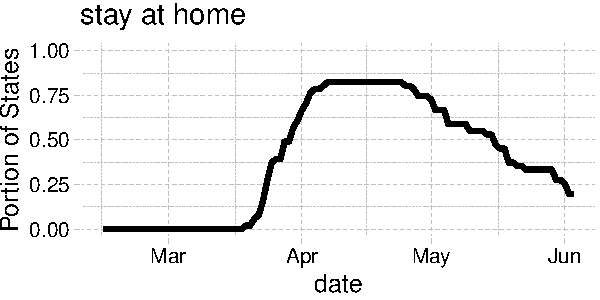
\includegraphics[width=0.33\textwidth]{pshelter_p}& \quad&
      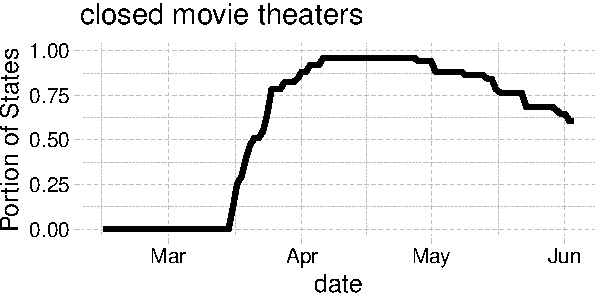
\includegraphics[width=0.33\textwidth]{pmovie_p}\\
        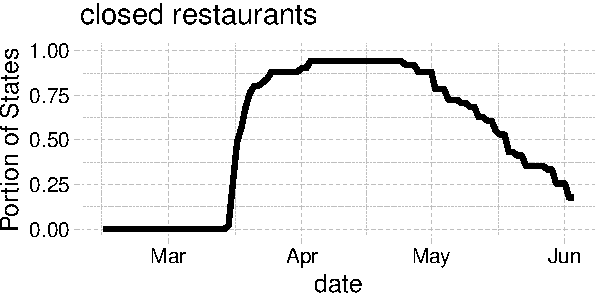
\includegraphics[width=0.33\textwidth]{prestaurant_p}
      & \quad&
        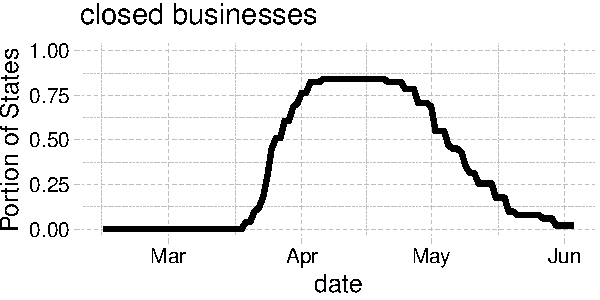
\includegraphics[width=0.33\textwidth]{pnonessential_p}
    \end{tabular}
  \end{minipage}
\end{figure}

 
\end{frame}
%----------------------------------------------------------------------------------------%


%%----------------------------------------------------------------------------------------%
%
\begin{frame}
  \frametitle{Correlations among policy and behavior variables}\vspace{-0.05cm}
  \begin{table}%\caption{Correlations among Policies and Behavior \label{tab:correlation}}\vspace{-0.2cm}
  \begin{minipage}{\linewidth}
    \resizebox{\linewidth}{!}{
   \begin{tabular}{lcccccccccc}
\toprule
\rotatebox{90}{ } & \rotatebox{90}{\bcolor  \textbf{workplaces}} & \rotatebox{90}{\bcolor \textbf{retail}} & \rotatebox{90}{\bcolor \textbf{grocery}} & \rotatebox{90}{\bcolor \textbf{transit}} & \rotatebox{90}{{\pcolor \textbf{masks for employees}}} & \rotatebox{90}{closed K-12 schools} & \rotatebox{90}{stay at home} & \rotatebox{90}{closed movie theaters} & \rotatebox{90}{closed restaurants} & \rotatebox{90}{closed businesses}\\
\midrule
workplaces & 1.00 &  &  &  &  &  &  &  &  & \\
retail & 0.94 & 1.00 &  &  &  &  &  &  &  & \\
grocery & 0.75 & 0.82 & 1.00 &  &  &  &  &  &  & \\
transit & 0.90 & 0.92 & 0.83 & 1.00 &  &  &  &  &  & \\
{\pcolor  \textbf{masks for employees}} & \textbf{\bcolor  -0.32} & \textbf{\bcolor   -0.19}& \textbf{\bcolor    -0.16} & \textbf{\bcolor   -0.30} & 1.00 &  &  &  &  & \\
\addlinespace
{\pcolor closed K-12 schools} & -0.92 & -0.81 & -0.58 & -0.75 &{\pcolor 0.46 }& 1.00 &  &  &  & \\
{\pcolor stay at home }& -0.70 & -0.69 & -0.71 & -0.72 & {\pcolor 0.31} &  0.65 & 1.00 &  &  & \\
{\pcolor closed movie theaters} & -0.82 & -0.77 & -0.65 & -0.72 & {\pcolor 0.40} & 0.85 & 0.75 & 1.00 &  & \\
{\pcolor closed restaurants }& -0.79 & -0.83 & -0.69 & -0.77 &{\pcolor 0.26} & 0.77 & 0.74 & 0.84 & 1.00 & \\
{\pcolor closed businesses} & -0.66 & -0.68 & -0.68 & -0.66 &{\pcolor 0.12} & 0.59 & 0.77 & 0.69 & 0.73 & 1.00\\
\bottomrule
\end{tabular}
    }\smallskip
       \begin{flushleft}
         \scriptsize
         Each off-diagonal entry reports a correlation coefficient of
         a pair of policy and behavior variables.
       \end{flushleft}
  \end{minipage}
\end{table} 



\end{frame}
%%----------------------------------------------------------------------------------------%



%----------------------------------------------------------------------------------------%

\begin{frame}
  \frametitle{Case and death growth conditional on \textbf{Mask Mandates }}\vspace{-0.05cm}



\begin{figure}[ht]
  %\caption{Case and death growth conditional on mask mandates \label{fig:masks}}\vspace{0.2cm}
  \begin{minipage}{\linewidth}
    \centering
    \begin{tabular}{cc}
      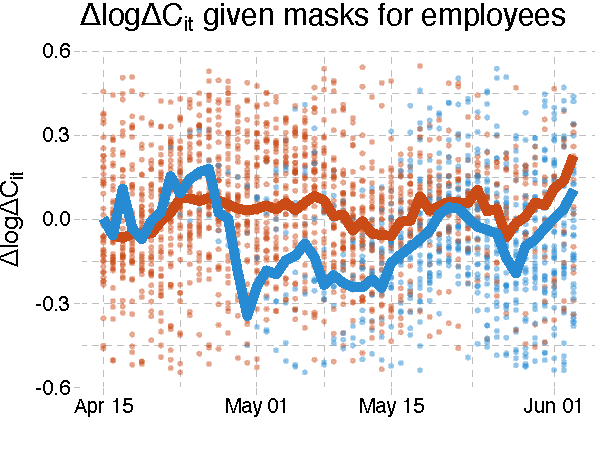
\includegraphics[width=0.5\textwidth]{pmaskbus-cases}
      &
        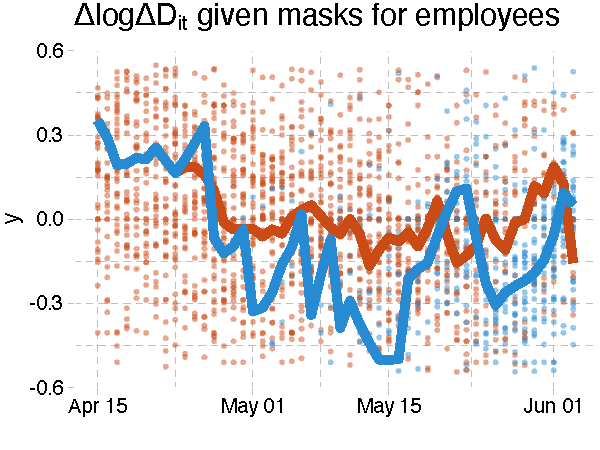
\includegraphics[width=0.5\textwidth]{pmaskbus-deaths} \\
    \textbf{Case Growth} &    \textbf{Death Growth} \\  
    \end{tabular}
%    \begin{flushleft}
%      \scriptsize In these figures, red points are the case or death
%      growth rate in states without a mask mandate. Blue points are
%      states with a mask mandate 14 (21 for deaths) days prior. The
%      red line is the average across states without a mask mandate 14
%      (21 for deaths) days earlier. The blue line is the average
%      across states with a mask mandate 14 (21 for deaths) earlier.
%    \end{flushleft}
  \end{minipage}
\end{figure}


\end{frame}
%----------------------------------------------------------------------------------------%


%%----------------------------------------------------------------------------------------%
%
%\begin{frame}
%  \frametitle{Case and death growth conditional on \textbf{Stay-at-Home Orders} }\vspace{-0.05cm}
%
%
%
%\begin{figure}[ht]
%  %\caption{Case and death growth conditional on mask mandates \label{fig:masks}}\vspace{0.2cm}
%  \begin{minipage}{\linewidth}
%    \centering
%    \begin{tabular}{cc}
%      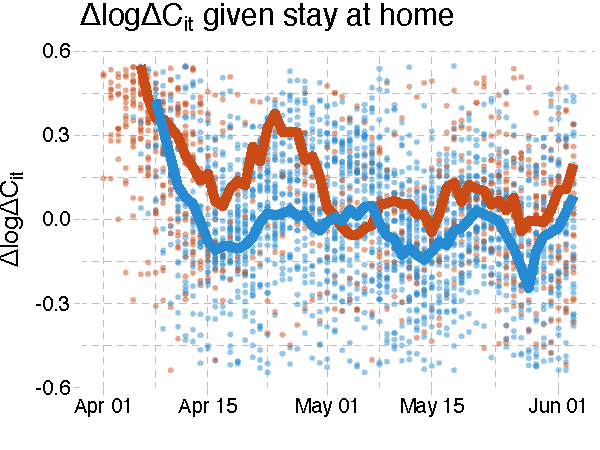
\includegraphics[width=0.5\textwidth]{pshelter-cases}
%      &
%        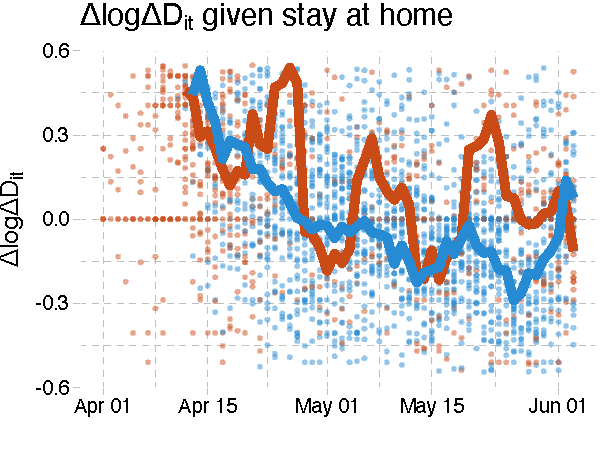
\includegraphics[width=0.5\textwidth]{pshelter-deaths} \\
%    \textbf{Case Growth} &    \textbf{Death Growth} \\  
%    \end{tabular}
%%    \begin{flushleft}
%%      \scriptsize In these figures, red points are the case or death
%%      growth rate in states without a mask mandate. Blue points are
%%      states with a mask mandate 14 (21 for deaths) days prior. The
%%      red line is the average across states without a mask mandate 14
%%      (21 for deaths) days earlier. The blue line is the average
%%      across states with a mask mandate 14 (21 for deaths) earlier.
%%    \end{flushleft}
%  \end{minipage}
%\end{figure}
%
%
%\end{frame}
%%----------------------------------------------------------------------------------------%

%----------------------------------------------------------------------------------------%

\begin{frame}
  \frametitle{Regression Analysis}

% We first examine how policies and information affect social distancing behaviors by estimating a version of (\ref{eq:R2}):
	\begin{align}
   &  {\ycolor  Y_{it+\ell}}
    = {\bcolor\alpha ' B_{it}} + {\pcolor\pi 'P_{it}} + {\icolor\mu'I_{it}} + {\wcolor\delta_Y 'W_{it}}  + \varepsilon^y_{it} \tag{BPI$\to$Y}\\
   % &  & \varepsilon^y_{it} \perp {\bcolor B_{it}}, {\pcolor P_{it}}, {\icolor I_{it}}, {\wcolor W_{it}} \label{eq:R1} \tag{BPI$\to$Y} \\
    &  {\bcolor B_{it}^j}
     =  {\pcolor \beta' P_{it}} + {\icolor \gamma'I_{it}} +  {\wcolor \delta_B' W_{it}} + \varepsilon^b_{it} \tag{PI$\to$B}\\
   \notag  \\
  % & & \varepsilon^b_{it} \perp {\pcolor P_{it}}, {\icolor I_{it}}, {\wcolor W_{it}}  \label{eq:R2} \tag{PI$\to$B} % \\
%    & {\pcolor P_{it}}
%    =  {\icolor\eta'I_{it}} + {\wcolor \delta_P' W_{it}} +   \varepsilon^p_{it},   & & \varepsilon^p_{it} \perp   {\icolor I_{it}}, {\wcolor W_{it}} \label{eq:R3}  \tag{I$\to$P}
 &  {\ycolor  Y_{it+\ell}}
   = ( {\pcolor\pi'}+ {\bcolor\alpha '}  {\pcolor \beta' }  )
    {\pcolor P_{it}} + (  {\icolor  \mu'}+{\bcolor\alpha '}  {\icolor \gamma'})
    {\icolor I_{it} }+ {\wcolor \bar \delta 'W_{it}}  + \bar \varepsilon_{it}. \tag{PI$\to$Y}
       \end{align}

\begin{itemize}
\item ${\ycolor Y_{it+\ell}}$:  the forward growth rate of cases or deaths\smallskip
\item   ${\bcolor B_{it}^j}$:  ``Transit,''  ``Workplaces''  ``Grocery," and ``Retail'' \smallskip
\item  $ {\pcolor  P_{it}} $:  various policies  lagged by 14 or 21 days\smallskip
\item $ {\icolor I_{it}} $: past cases/deaths,  national-level cases/deaths etc.\smallskip
\item $ {\wcolor   W_{it}}$: state-level characteristics, month dummies, and their interactions.
\end{itemize}


\end{frame}
%----------------------------------------------------------------------------------------%
 


%----------------------------------------------------------------------------------------%

\begin{frame}
  \frametitle{The Effect of Policies and Information on Behavior (PI$\to$ B)}

  % \textbf{Plan: will only present (5)-(8) columns}
  % behavior-deathsinfo-nationinfo-pib is columns (5)-(8)
  % behavior-deathsinfo-stateinfo-pib is columns (1)-(4)
  % for cases:
  % behavior-cases-nationinfo-pib is columns (5)-(8)
  % behavior-cases-stateinfo-pib is columns (1)-(4)
  
  
\begin{table}[!htbp] \centering
% \caption{The Direct Effect of Behavior and Policies on Case and
%   Death Growth ($PBI \to Y$)}\vspace{-0.3cm}
 \begin{minipage}{\linewidth}
   \centering
   \resizebox*{!}{\dimexpr\textheight-2\baselineskip\relax}{
     \scriptsize       \begin{tabular}{@{\extracolsep{1pt}}lcccc} 
\\[-1.8ex]\hline 
\hline \\[-1.8ex] 
 & \multicolumn{4}{c}{\textit{Dependent variable:}} \\ 
\cline{2-5} 
 &{\bcolor  Workplaces} &  {\bcolor  Transit }&{\bcolor  Workplaces} &{\bcolor   Transit }\\ 
\\[-1.8ex] & (1) & (2) & (3) & (4)  \\ 
\hline \\[-1.8ex]  
%{\pcolor Mask for Employees}&$-$0.011 & $-$3.104 & $-$0.812 & $-$4.044$^{*}$ \\ 
%  & (-0.873)& (-2.213)& (-0.660)& (2.094) \\ 
%{\pcolor School Closures} & $-$19.678$^{***}$ & $-$22.694$^{***}$ & $-$4.908$^{***}$ & $-$5.147 \\ 
%  & (-2.83& (-5.597& (-1.526& (4.868) \\ 
%{\pcolor Stay-at-Home} & $-$2.943$^{***}$ & $-$8.577$^{***}$ & $-$3.222$^{***}$ & $-$8.881$^{***}$ \\ 
%  & (-1.045)& (-2.366)& (-0.957)& (2.347) \\ 
% \quad\qquad $\vdots$ &$\vdots$ &$\vdots$ &$\vdots$    \\\hline  
%  {\icolor  $\Delta \log \Delta C_{it}$} & 1.791$^{***}$ & 1.857$^{***}$ & 1.596$^{***}$ & 1.591$^{***}$ \\ 
%  & (-0.356)& (-0.553)& (-0.221)& (0.601) \\ 
% {\icolor   $\log \Delta C_{it}$} & $-$2.107$^{***}$ & $-$1.092 & $-$0.366 & 0.997 \\ 
%  & (-0.493)& (-1.175)& (-0.340)& (1.285) \\ 
% {\icolor $\Delta \log \Delta C_{it}$.national }&  &  & $-$2.998$^{***}$ & $-$3.294$^{***}$ \\ 
%  &  &  & (-0.452)& (1.187) \\ 
%  {\icolor $\log \Delta C_{it}$.national} &  &  & $-$6.610$^{***}$ & $-$7.854$^{***}$ \\ 
%  &  &  & (-0.440)& (1.396) \\  
%\hline \\[-1.8ex]		
%{\pcolor $\sum_j \mathrm{Policy}_j$} &{\pcolor  -29.699$^{***}$} & {\pcolor -42.515$^{***}$} &{\pcolor -13.972$^{***}$}& {\pcolor -23.772$^{***}$} \\ 
% & (-3.296)& (-6.813)& (-1.953)& (5.127) \\  \hline 
% 
% 
 
{\pcolor Mask for Employees}&0.023$^{*}$&0.015&0.005&$-$0.010 \\ 
  &(0.012)&(0.025)&(0.008)&(0.023) \\ 
{\pcolor School Closures} &$-$0.196$^{***}$ &$-$0.243$^{***}$ &$-$0.044$^{***}$ &$-$0.047 \\ 
  &(0.030)&(0.050)&(0.013&(0.041) \\ 
{\pcolor Stay-at-Home} &$-$0.028$^{**}$ &$-$0.062$^{**}$ &$-$0.034$^{***}$ &$-$0.074$^{***}$ \\ 
  &(0.013)&(0.028)&(0.011)&(0.028) \\ 
{\pcolor Business Closures} &$-$0.081$^{***}$ &$-$0.080$^{**}$ &$-$0.049$^{***}$ &$-$0.042 \\ 
  &(0.017)&(0.038)&(0.012)&(0.036) \\  \hline
  ${\pcolor \sum_j \mathrm{Policy}_j}$ &{\pcolor  -0.282$^{***}$}  &{\pcolor  -0.371$^{***}$ }&{\pcolor  -0.122$^{***}$}   & {\pcolor -0.172$^{***}$ }\\ 
    & (0.041) &   (0.078) & (0.022)  & (0.060) \\ \hline
   {\icolor $\Delta \log \Delta C_{it}$} &0.015$^{***}$ &0.014$^{***}$ &0.017$^{***}$ &0.020$^{***}$ \\ 
  &(0.003)&(0.005 )&(0.002)&(0.005) \\ 
  {\icolor  $\log \Delta C_{it}$} & {\icolor$-$0.024$^{***}$} & {\icolor$-$0.018$^{*}$} &$-$0.005 &0.004 \\ 
  &(0.005)&(0.010)&(0.004)&(0.011) \\ 
   {\icolor $\Delta \log \Delta C_{it}$.national}& &  &$-$0.033$^{***}$ &$-$0.053$^{***}$ \\ 
 & &  &(0.005)&(0.012) \\ 
 {\icolor   $\log \Delta C_{it}$.national}& &  &$-$0.072$^{***}$ &$-$0.091$^{***}$ \\ 
 & &  &(0.004)&(0.012) \\ \hline

\hline \\[-1.8ex]  
\end{tabular}  }
% \begin{flushleft}
%     \scriptsize Dependent variable is the weekly growth rate of
%     confirmed cases (in the left panel) or deaths (in the right
%     panel) as defined in equation (\ref{eq:y}). The covariates
%     include lagged policy and behavior variables, which are
%     constructed as 7 day moving averages between $t$ to $t-7$ of
%     corresponding daily measures.  The row
%     ``$\sum_j \mathrm{Policies}_j$'' reports the sum of six policy
%     coefficients.  The row ``$\sum_k w_k \mathrm{Behavior}_k$''
%     reports the sum of four coefficients of behavior variables
%     weighted by the average of each behavioral variable from April
%     1st-10th.
%   \end{flushleft}
 \end{minipage} \vspace{-0.4cm}
  \begin{flushleft}
\tiny
Other policies include closures of movie theaters, restaurants, and non-essential businesses. State characteristics, month dummies, and their interactions are included.
\end{flushleft}
\end{table}

 
\end{frame}
%----------------------------------------------------------------------------------------%



%----------------------------------------------------------------------------------------%

\begin{frame}
  \frametitle{The Direct Effect of Policies, Behavior, and Information on Case Growth (BPI$\to$Y)}

%\textbf{Plan: will only present (1) and (3) columns for each table, possibly only for death growth}


\begin{table}[!htbp] \centering
% \caption{The Direct Effect of Behavior and Policies on Case and
%   Death Growth ($PBI \to Y$)}\vspace{-0.3cm}
 \label{tab:BPItoY}
 \begin{minipage}{\linewidth}
   \centering
   \resizebox*{!}{\dimexpr\textheight-2\baselineskip\relax}{
     \scriptsize

\begin{tabular}{@{\extracolsep{1pt}}lcccc} 
\\[-1.8ex]\hline 
\hline \\[-1.8ex] 
 & \multicolumn{4}{c}{\textit{Dependent variable:\ $ \boldsymbol{\Delta \log \Delta C_{it}}$}} \\ 
\cline{2-5} 
% & \multicolumn{4}{c}{$\Delta \log \Delta C_{it}$} \\ 
\\[-1.8ex] & (1) & (2) & (3) & (4)\\ 
\hline \\[-1.8ex] 
{\pcolor lag(masks for employees, 14) }& $-$0.090$^{***}$ & $-$0.091$^{***}$ & $-$0.100$^{***}$ & $-$0.100$^{***}$ \\ 
  & (0.031) & (0.032) & (0.029) & (0.030) \\ 
 {\pcolor  lag(closed K-12 schools, 14)} & $-$0.074 & $-$0.083 & 0.043 & 0.031 \\ 
  & (0.080) & (0.090) & (0.096) & (0.103) \\ 
%  lag(stay at home, 14) & $-$0.063 & $-$0.058 & $-$0.079 & $-$0.071 \\ 
%  & (0.050) & (0.048) & (0.052) & (0.050) \\ 
  
& $\vdots$ &$\vdots$ &$\vdots$ &$\vdots$    \\\hline
%  lag(business closure policies, 14) & 0.051 &  & 0.045 &  \\ 
%  & (0.062) &  & (0.060) &  \\ 
%  lag(closed movie theaters, 14) &  & 0.032 &  & 0.045 \\ 
%  &  & (0.050) &  & (0.049) \\ 
%  lag(closed restaurants, 14) &  & 0.023 &  & 0.022 \\ 
%  &  & (0.044) &  & (0.043) \\ 
%  lag(closed non-essent bus, 14) &  & $-$0.001 &  & $-$0.016 \\ 
%  &  & (0.040) &  & (0.040) \\ 
    {\bcolor  lag(workplaces, 14)} & 1.055$^{*}$ & 1.042$^{*}$ & 0.391 & 0.355 \\ 
  & (0.543) & (0.556) & (0.610) & (0.618) \\ 
  {\bcolor  lag(retail, 14)} & 0.594$^{*}$ & 0.611$^{**}$ & 0.316 & 0.342 \\ 
  & (0.303) & (0.309) & (0.316) & (0.317) \\ 
  {\bcolor  lag(grocery, 14) }& $-$0.471$^{*}$ & $-$0.478$^{*}$ & $-$0.259 & $-$0.266 \\ 
  & (0.284) & (0.288) & (0.282) & (0.284) \\ 
  {\bcolor  lag(transit, 14)} & 0.347 & 0.339 & 0.355 & 0.339 \\ 
  & (0.258) & (0.268) & (0.247) & (0.253) \\  \hline \hline
  {\bcolor  $\sum_k w_k \mathrm{Behavior}_k$ }&  {\bcolor -0.804$^{***}$} &  {\bcolor -0.801$^{***}$} & {\bcolor  -0.425$^{***}$} &  {\bcolor -0.413$^{***}$} \\ 
 & (0.140) & (0.140) & (0.157) & (0.160) \\ %Observations & 3,823 & 3,823 & 3,823 & 3,823 \\ 
 \hline \hline
  lag($\Delta \log \Delta C_{it}$, 14) & 0.015 & 0.015 & 0.024 & 0.024 \\ 
  & (0.026) & (0.025) & (0.028) & (0.028) \\ 
   {\icolor  lag($\log \Delta C_{it}$, 14) }&   {\icolor $-$0.105$^{***}$} &   {\icolor $-$0.105$^{***}$} &   {\icolor $-$0.088$^{***}$} &   {\icolor $-$0.087$^{***}$} \\ 
  & (0.019) & (0.019) & (0.021) & (0.021) \\ 
  lag($\Delta \log \Delta C_{it}$.national, 14) &  &  & $-$0.095$^{**}$ & $-$0.095$^{**}$ \\ 
  &  &  & (0.042) & (0.043) \\ 
  lag($\log \Delta C_{it}$.national, 14) &  &  & $-$0.177$^{***}$ & $-$0.180$^{***}$ \\ 
  &  &  & (0.049) & (0.050) \\ 
  $\Delta \log T_{it}$ & 0.152$^{***}$ & 0.153$^{***}$ & 0.155$^{***}$ & 0.156$^{***}$ \\ 
  & (0.043) & (0.043) & (0.042) & (0.041) \\ 
 \hline \\[-1.8ex] 
%state variables & Yes & Yes & Yes & Yes \\ 
%Month $\times$ state variables & Yes & Yes & Yes & Yes \\ 
%\hline \\[-1.8ex] 
%%$\sum_j \mathrm{Policy}_j$ & -0.176 & -0.178 & -0.091 & -0.090 \\ 
%% & (0.128) & (0.133) & (0.153) & (0.158) \\ 
%
%%R$^{2}$ & 0.759 & 0.759 & 0.765 & 0.765 \\ 
%%Adjusted R$^{2}$ & 0.757 & 0.757 & 0.762 & 0.762 \\ 
%\hline 
%\hline \\[-1.8ex] 
%\textit{Note:}  & \multicolumn{4}{r}{$^{*}$p$<$0.1; $^{**}$p$<$0.05; $^{***}$p$<$0.01} \\ 
\end{tabular} 
   }
% \begin{flushleft}
%     \scriptsize Dependent variable is the weekly growth rate of
%     confirmed cases (in the left panel) or deaths (in the right
%     panel) as defined in equation (\ref{eq:y}). The covariates
%     include lagged policy and behavior variables, which are
%     constructed as 7 day moving averages between $t$ to $t-7$ of
%     corresponding daily measures.  The row
%     ``$\sum_j \mathrm{Policies}_j$'' reports the sum of six policy
%     coefficients.  The row ``$\sum_k w_k \mathrm{Behavior}_k$''
%     reports the sum of four coefficients of behavior variables
%     weighted by the average of each behavioral variable from April
%     1st-10th.
%   \end{flushleft}
 \end{minipage}
  \begin{flushleft}
\tiny
Other policies include closures of movie theaters, restaurants, and non-essential businesses. State characteristics, month dummies, and their interactions are included.
\end{flushleft}
\end{table}
\end{frame}
%----------------------------------------------------------------------------------------%




%----------------------------------------------------------------------------------------%

\begin{frame}
  \frametitle{Direct and Indirect Policy Effects for Case Regression}

\begin{table}
 % \caption{\label{tab:dieff}Direct and Indirect Policy Effects}
\begin{minipage}{\linewidth}
  \centering
    \tiny
  \begin{tabular}{c}
%    \textbf{Cases}
%    \\
%    \input{tables_and_figures/dieff-cases}
      \\
    \textbf{{\normalsize Case Growth Regression \underline{without national case variables}}}
    \\
    \\
\begin{tabular}{lccc|c|c|c}
\toprule
&\multicolumn{3}{c|}{ PI$\to$B Coef.\ \& \ PBI$\to$Y Coef.  } &PI$\to$Y Coef.&Average &Difference  \\
  & Direct & Indirect & Total & Total & Total & (over-id test) \\\
  &${\pcolor\pi'}$&${\bcolor\alpha '}  {\pcolor \beta' }$ &${\pcolor\pi'}+{\bcolor\alpha '}  {\pcolor \beta' }$ &${\pcolor\pi'}+{\bcolor\alpha '}  {\pcolor \beta' }$ & ${\pcolor\pi'}+{\bcolor\alpha '}  {\pcolor \beta' }$&  \\
\midrule
Mask for Employees &\alert{  -0.096$^{***}$} & ---- & \alert{ -0.096$^{***}$} & \alert{ -0.083$^{**}$} & \alert{ -0.089$^{***}$} &\alert{  -0.013}\\
 & (0.030) & --- & (0.030) & (0.039) & (0.032) & (0.025)\\
School Closures  & -0.073 & -0.364$^{***}$ & -0.436$^{***}$ & -0.226$^{**}$ & -0.331$^{***}$ & -0.210$^{***}$\\
 & (0.078) & (0.094) & (0.119) & (0.092) & (0.102) & (0.056)\\
Stay-at-Home  & -0.053 & -0.032 & -0.085 & -0.127$^{**}$ & -0.106$^{*}$ & 0.042$^{**}$\\
 & (0.052) & (0.028) & (0.058) & (0.057) & (0.057) & (0.020)\\
Business Closures & --- & -0.157$^{***}$ & -0.157$^{***}$ & -0.076 & -0.117$^{**}$ & -0.081\\
 & --- & (0.042) & (0.042) & (0.066) & (0.048) & (0.054)\\
 
%Mask for Employees& \alert{ -0.084$^{**}$} &\alert{  -0.008} & \alert{ -0.092$^{**}$} & \alert{ -0.081$^{**}$} &\alert{  -0.086$^{**}$} & \alert{-0.011}\\
% & (0.034) & (0.024) & (0.044) & (0.040) & (0.041) & (0.015)\\
%School Closures & -0.095 & -0.337$^{***}$ & -0.432$^{***}$ & -0.240$^{**}$ & -0.336$^{***}$ & -0.192$^{***}$\\
% & (0.093) & (0.091) & (0.118) & (0.095) & (0.105) & (0.047)\\
%Stay-at-Home & -0.041 & -0.065$^{**}$ & -0.106$^{**}$ & -0.126$^{**}$ & -0.116$^{**}$ & 0.020\\
% & (0.046) & (0.031) & (0.053) & (0.055) & (0.054) & (0.013)\\  
 \quad\qquad $\vdots$ &$\vdots$ &$\vdots$ &$\vdots$ &$\vdots$ &$\vdots$ &$\vdots$  \\\hline
%Movie Closures & 0.049 & -0.024 & 0.024 & 0.030 & 0.027 & -0.005\\
% & (0.048) & (0.025) & (0.055) & (0.050) & (0.052) & (0.016)\\
%Restaurants  Cl.& 0.020 & -0.091$^{***}$ & -0.071 & -0.042 & -0.057 & -0.029$^{*}$\\
% & (0.046) & (0.029) & (0.044) & (0.048) & (0.045) & (0.016)\\
%Non-essential Bus. & -0.004 & -0.024 & -0.028 & -0.048 & -0.038 & 0.020$^{*}$\\
% & (0.041) & (0.019) & (0.049) & (0.050) & (0.049) & (0.011)\\ \hline
%$\sum_j \mathrm{Policy}_j$ & -0.155 & -0.550$^{***}$ & -0.704$^{***}$ & -0.508$^{***}$ & -0.606$^{***}$ & -0.196$^{***}$\\
% & (0.136) & (0.140) & (0.188) & (0.157) & (0.171) & (0.052)\\
 $\sum_j \mathrm{Policy}_j$ & -0.221$^{**}$ & -0.553$^{***}$ & -0.774$^{***}$ & -0.512$^{***}$ & -0.643$^{***}$ & -0.262$^{***}$\\
 & (0.108) & (0.124) & (0.166) & (0.151) & (0.156) & (0.061)\\

%$\Delta \log \Delta C_{it}$ & 0.017 & 0.023$^{**}$ & 0.040$^{*}$ & 0.040$^{*}$ & 0.040$^{*}$ & 0.000\\
% & (0.025) & (0.010) & (0.023) & (0.024) & (0.023) & (0.006)\\
%$\log \Delta C_{it}$ & -0.110$^{***}$ & -0.036$^{**}$ & -0.146$^{***}$ & -0.138$^{***}$ & -0.142$^{***}$ & -0.008\\
% & (0.019) & (0.014) & (0.026) & (0.023) & (0.024) & (0.007)\\ 
\bottomrule
\end{tabular}     \\
  \end{tabular}
%  \smallskip
%  \begin{flushleft}
%      \scriptsize Direct effects capture the effect of policy on case
%      growth holding behavior, information, and confounders
%      constant. Direct effects are given by ${\pcolor \pi}$ in
%      equation (\ref{eq:R1}). Indirect effects capture how policy
%      changes behavior and behavior shift case growth. They are given
%      by ${\bcolor \alpha}$ from (\ref{eq:R1}) times ${\pcolor \beta}$
%      from (\ref{eq:R2}). The total effect is
%      ${\pcolor \pi} + {\pcolor \beta} {\bcolor \alpha}$. Column
%      ``PI$\to$Y Coefficients'' shows the coefficient estimates from
%      \ref{eq:R4}. Columns ``Difference''    are  the differences between
%      the estimates from (\ref{eq:R4}) and the combination of
%      (\ref{eq:R1}) and (\ref{eq:R2}) while column ``Average'' are their averages.
%      Standard errors are computed by
%      bootstrap and clustered on state.
%    %  \ref{tab:PtoY}.
%    \end{flushleft}
  \end{minipage}
\end{table}
\begin{flushleft}
\tiny
State characteristics, month dummies, and their interactions are included.
\end{flushleft}
\end{frame}
%----------------------------------------------------------------------------------------%


%----------------------------------------------------------------------------------------%

\begin{frame}
  \frametitle{Direct and Indirect Policy Effects for Case Regression}

\begin{table}
 % \caption{\label{tab:dieff}Direct and Indirect Policy Effects}
\begin{minipage}{\linewidth}
  \centering
    \tiny
  \begin{tabular}{c}
%    \textbf{Cases}
%    \\
%    \input{tables_and_figures/dieff-cases}
      \\
    \textbf{{\normalsize Case Growth Regression \underline{with national case variables}}}
    \\
    \\
\begin{tabular}{lccc|c|c|c}
\toprule
&\multicolumn{3}{c|}{ PI$\to$B Coef.\ \& \ PBI$\to$Y Coef.  } &PI$\to$Y Coef.& Average & Difference \\
  & Direct & Indirect & Total & Total & Total &   (over-id test)\\\
  &${\pcolor\pi'}$&${\bcolor\alpha '}  {\pcolor \beta' }$ &${\pcolor\pi'}+{\bcolor\alpha '}  {\pcolor \beta' }$ &${\pcolor\pi'}+{\bcolor\alpha '}  {\pcolor \beta' }$ & ${\pcolor\pi'}+{\bcolor\alpha '}  {\pcolor \beta' }$&  \\
\midrule
Mask for Employees &\alert{ -0.105$^{***}$ }& --- & \alert{-0.105$^{***}$} & \alert{-0.103$^{***}$} & \alert{-0.104$^{***}$} &\alert{ -0.001}\\
 & (0.027) & --- & (0.027) & (0.031) & (0.028) & (0.016)\\
School Closures & 0.045 & -0.022 & 0.023 & 0.029 & 0.026 & -0.007\\
 & (0.092) & (0.034) & (0.101) & (0.099) & (0.100) & (0.015)\\
Stay-at-Home & -0.071 & -0.033$^{*}$ & -0.104$^{*}$ & -0.115$^{**}$ & -0.110$^{**}$ & 0.011\\
 & (0.052) & (0.019) & (0.056) & (0.052) & (0.053) & (0.017)\\
Business closures & --- & -0.038 & -0.038 & -0.001 & -0.019 & -0.038\\
 &---& (0.024) & (0.024) & (0.061) & (0.038) & (0.054)\\
 \quad\qquad $\vdots$ &$\vdots$ &$\vdots$ &$\vdots$ &$\vdots$ &$\vdots$ &$\vdots$  \\\hline
$\sum_j \mathrm{Policy}_j$ & -0.131 & -0.094$^{*}$ & -0.225$^{*}$ & -0.190 & -0.207 & -0.035\\
 & (0.123) & (0.049) & (0.134) & (0.155) & (0.143) & (0.047)\\
 
 
%Mask for Employees& \alert{-0.097$^{***}$} & \alert{ -0.019} & \alert{ -0.116$^{***}$} &  \alert{-0.105$^{***}$} & \alert{ -0.111$^{***}$} &  \alert{-0.011}\\
% & (0.033) & (0.017) & (0.040) & (0.038) & (0.039) & (0.011)\\
%School Closures & 0.025 & -0.021 & 0.004 & 0.009 & 0.007 & -0.005\\
% & (0.103) & (0.040) & (0.110) & (0.108) & (0.109) & (0.015)\\
%Stay-at-Home  & -0.064 & -0.047$^{**}$ & -0.112$^{**}$ & -0.117$^{**}$ & -0.114$^{**}$ & 0.005\\
% & (0.047) & (0.023) & (0.049) & (0.049) & (0.049) & (0.009)\\ 
% \quad\qquad $\vdots$ &$\vdots$ &$\vdots$ &$\vdots$ &$\vdots$ &$\vdots$ &$\vdots$  \\\hline 
%%closed movie theaters & 0.053 & -0.002 & 0.051 & 0.058 & 0.055 & -0.006\\
%% & (0.048) & (0.017) & (0.048) & (0.046) & (0.047) & (0.011)\\
%%closed restaurants & 0.021 & -0.038$^{*}$ & -0.017 & -0.010 & -0.013 & -0.008\\
%% & (0.045) & (0.020) & (0.041) & (0.043) & (0.041) & (0.011)\\
%%closed businesses & -0.016 & -0.013 & -0.028 & -0.035 & -0.032 & 0.006\\
%% & (0.042) & (0.012) & (0.044) & (0.044) & (0.044) & (0.008)\\
%$\sum_j \mathrm{Policy}_j$ & -0.078 & -0.140$^{**}$ & -0.218 & -0.199 & -0.209 & -0.019\\
% & (0.160) & (0.065) & (0.168) & (0.166) & (0.167) & (0.018)\\
%$\Delta \log \Delta C_{it}$ & 0.023 & 0.010 & 0.033 & 0.033 & 0.033 & -0.000\\
% & (0.028) & (0.007) & (0.028) & (0.028) & (0.028) & (0.003)\\
%$\log \Delta C_{it}$ & -0.089$^{***}$ & 0.001 & -0.088$^{***}$ & -0.091$^{***}$ & -0.090$^{***}$ & 0.003\\
% & (0.021) & (0.011) & (0.028) & (0.027) & (0.027) & (0.005)\\
%$\Delta \log \Delta C_{it}$.national & -0.090$^{**}$ & -0.040$^{**}$ & -0.130$^{***}$ & -0.123$^{***}$ & -0.126$^{***}$ & -0.006\\
% & (0.044) & (0.016) & (0.044) & (0.042) & (0.042) & (0.013)\\
%$\log \Delta C_{it}$.national & -0.184$^{***}$ & -0.068$^{***}$ & -0.252$^{***}$ & -0.241$^{***}$ & -0.247$^{***}$ & -0.010\\
% & (0.047) & (0.022) & (0.044) & (0.044) & (0.044) & (0.010)\\
\bottomrule
\end{tabular}     \\
  \end{tabular}
%  \smallskip
%  \begin{flushleft}
%      \scriptsize Direct effects capture the effect of policy on case
%      growth holding behavior, information, and confounders
%      constant. Direct effects are given by ${\pcolor \pi}$ in
%      equation (\ref{eq:R1}). Indirect effects capture how policy
%      changes behavior and behavior shift case growth. They are given
%      by ${\bcolor \alpha}$ from (\ref{eq:R1}) times ${\pcolor \beta}$
%      from (\ref{eq:R2}). The total effect is
%      ${\pcolor \pi} + {\pcolor \beta} {\bcolor \alpha}$. Column
%      ``PI$\to$Y Coefficients'' shows the coefficient estimates from
%      \ref{eq:R4}. Columns ``Difference''    are  the differences between
%      the estimates from (\ref{eq:R4}) and the combination of
%      (\ref{eq:R1}) and (\ref{eq:R2}) while column ``Average'' are their averages.
%      Standard errors are computed by
%      bootstrap and clustered on state.
%    %  \ref{tab:PtoY}.
%    \end{flushleft}
  \end{minipage}
\end{table}
\begin{flushleft}
\tiny
Other policies include closures of movie theaters, restaurants, and non-essential businesses.  State characteristics, month dummies, and their interactions are included.

\end{flushleft}
\end{frame}
%----------------------------------------------------------------------------------------%

%%----------------------------------------------------------------------------------------%
%
%\begin{frame}
%  \frametitle{Direct and Indirect Policy Effects for Death Regression}
%
%\begin{table}
% % \caption{\label{tab:dieff}Direct and Indirect Policy Effects}
%\begin{minipage}{\linewidth}
%  \centering
%    \tiny
%  \begin{tabular}{c}
%%    \textbf{Cases}
%%    \\
%%    \input{tables_and_figures/dieff-cases}
%      \\
%    \textbf{{\normalsize Death Growth Regression  \underline{without national death variables}}}
%    \\
%    \\
%\begin{tabular}{lccc|c|c|c}
%\toprule
%&\multicolumn{3}{c|}{ PI$\to$B Coef.\ \& \ PBI$\to$Y Coef.  } &PI$\to$Y Coef. & Average& Difference\\
%  & Direct & Indirect & Total & Total  & Total& (over-id test)  \\\
%  &${\pcolor\pi'}$&${\bcolor\alpha '}  {\pcolor \beta' }$ &${\pcolor\pi'}+{\bcolor\alpha '}  {\pcolor \beta' }$ &${\pcolor\pi'}+{\bcolor\alpha '}  {\pcolor \beta' }$ &  ${\pcolor\pi'}+{\bcolor\alpha '}  {\pcolor \beta' }$& \\
%\midrule
%Mask for Employees & \alert{  -0.145$^{***}$} & \alert{  -0.004} &  \alert{ -0.149$^{***}$} & \alert{  -0.133$^{***}$} &  \alert{ -0.141$^{***}$} & \alert{  -0.016}\\
% & (0.050) & (0.023) & (0.055) & (0.051) & (0.052) & (0.015)\\
%School Closures & -0.271$^{***}$ & -0.451$^{***}$ & -0.722$^{***}$ & -0.641$^{***}$ & -0.681$^{***}$ & -0.081$^{***}$\\
% & (0.092) & (0.082) & (0.111) & (0.107) & (0.108) & (0.026)\\
%Stay-at-Home & -0.040 & -0.034 & -0.074 & -0.080 & -0.077 & 0.006\\
% & (0.064) & (0.035) & (0.064) & (0.064) & (0.064) & (0.015)\\ \hline
%%closed movie theaters & 0.039 & -0.025 & 0.014 & 0.018 & 0.016 & -0.004\\
%% & (0.091) & (0.030) & (0.089) & (0.089) & (0.088) & (0.018)\\
%%closed restaurants & 0.085 & -0.105$^{**}$ & -0.020 & -0.015 & -0.018 & -0.005\\
%% & (0.065) & (0.042) & (0.056) & (0.057) & (0.056) & (0.016)\\
%%closed businesses & -0.003 & -0.024 & -0.027 & -0.038 & -0.032 & 0.011\\
%% & (0.055) & (0.021) & (0.061) & (0.063) & (0.062) & (0.013)\\
%$\sum_j \mathrm{Policy}_j$ & -0.334$^{**}$ & -0.644$^{***}$ & -0.979$^{***}$ & -0.889$^{***}$ & -0.934$^{***}$ & -0.090$^{**}$\\
% & (0.160) & (0.154) & (0.171) & (0.165) & (0.167) & (0.035)\\
%%$\Delta \log \Delta D_{it}$ & 0.016 & -0.025$^{**}$ & -0.009 & -0.000 & -0.004 & -0.009$^{*}$\\
%% & (0.034) & (0.011) & (0.031) & (0.032) & (0.031) & (0.005)\\
%%$\log \Delta D_{it}$ & -0.051$^{**}$ & -0.018$^{*}$ & -0.069$^{**}$ & -0.078$^{***}$ & -0.073$^{***}$ & 0.009$^{*}$\\
%% & (0.024) & (0.010) & (0.028) & (0.026) & (0.027) & (0.005)\\
%\bottomrule
%\end{tabular}
%    \\
%  \end{tabular}
%%  \smallskip
%%  \begin{flushleft}
%%      \scriptsize Direct effects capture the effect of policy on case
%%      growth holding behavior, information, and confounders
%%      constant. Direct effects are given by ${\pcolor \pi}$ in
%%      equation (\ref{eq:R1}). Indirect effects capture how policy
%%      changes behavior and behavior shift case growth. They are given
%%      by ${\bcolor \alpha}$ from (\ref{eq:R1}) times ${\pcolor \beta}$
%%      from (\ref{eq:R2}). The total effect is
%%      ${\pcolor \pi} + {\pcolor \beta} {\bcolor \alpha}$. Column
%%      ``PI$\to$Y Coefficients'' shows the coefficient estimates from
%%      \ref{eq:R4}. Columns ``Difference''    are  the differences between
%%      the estimates from (\ref{eq:R4}) and the combination of
%%      (\ref{eq:R1}) and (\ref{eq:R2}) while column ``Average'' are their averages.
%%      Standard errors are computed by
%%      bootstrap and clustered on state.
%%    %  \ref{tab:PtoY}.
%%    \end{flushleft}
%  \end{minipage}
%\end{table}
%\begin{flushleft}
%\footnotesize
%Other policies include closures of movie theaters, restaurants, and non-essential businesses.
%\end{flushleft}
%\end{frame}
%%----------------------------------------------------------------------------------------%




%----------------------------------------------------------------------------------------%

\begin{frame}
  \frametitle{Sensitivity Analysis}
  

  \begin{itemize} 
  \item[(1)] Baseline
  \item[(2)]  Exclude  the state of New York
  \item[(3)]   Add \% of people wearing masks in March and April
   \item[(4)]   Add the log of Trump's vote share  in 2016
    \item[(5)]   Add  past behavior variables  as information
   \item[(6)]   All of (2)-(5)
   \item[(7)] Add weekly dummies
   \item[(8)] Instrumenting $\Delta \log T_{it}$ with one week lagged  log value.
   \item[(9)]   Double Machine Learning (DML) with Lasso in (3)-(5).    
    \item[(10)]  DML with Random Forest  in (3)-(5).      %  \item[(10)]   Add latent state confounders and weekly dummies as components of $W_{it}$, estimated using fixed effects with bias correction.
    \item Fixed effects + weekly dummies
    \item 
  Alternative Timing assumption ($\ell=10$ for cases and $\ell=23$ for deaths) on all of the above.
  \end{itemize}  
\end{frame}
%----------------------------------------------------------------------------------------%

%----------------------------------------------------------------------------------------% 

\begin{frame}
  \frametitle{Sensitivity Analysis: Mask Mandates and Stay-at-Home}
  
  
  \begin{figure}[ht]
%  \caption{Estimated Coefficients for  Policy Variables: Sensitivity Analysis \label{fig:whisker}}\bigskip
  \begin{minipage}{\linewidth}
    \centering
%   {\textbf{(A)  masks for employees}}\\
%    \medskip
    \begin{tabular}{cc}
 $\quad$ Mask Mandates &$\quad$  Stay-at-Home Orders\\
      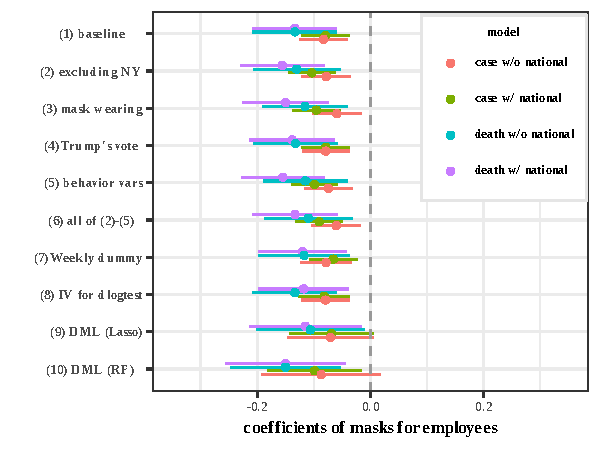
\includegraphics[width=0.49\textwidth]{tables_and_figures/pmaskbus-whisker-14}
      &
      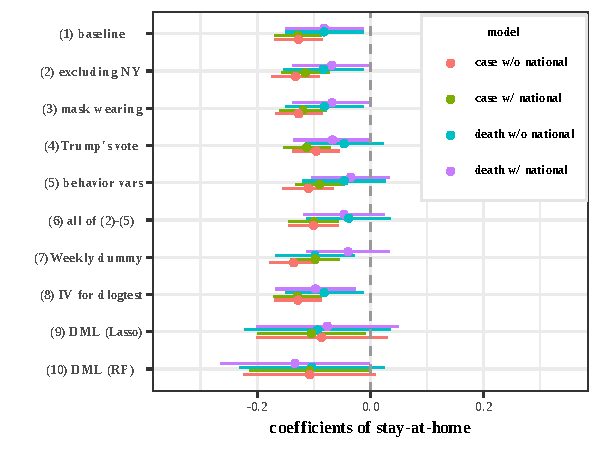
\includegraphics[width=0.49\textwidth]{tables_and_figures/pshelter-whisker-14}\qquad
    \end{tabular}
  \end{minipage} %\\\smallskip
%    \begin{minipage}{\linewidth}
%    \centering
%     {\textbf{(B)  closed K-12 Schools}}\\
%    \medskip
%    \begin{tabular}{cc}
% $\quad$  (i) baseline timing$^\dagger$ &$\quad$ (ii) alternative timing$^\ddagger$\\
%      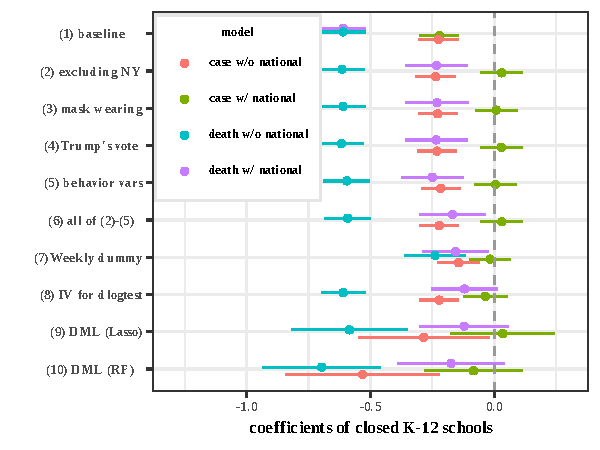
\includegraphics[width=0.5\textwidth]{tables_and_figures/pk12-whisker-14}
%      &
%      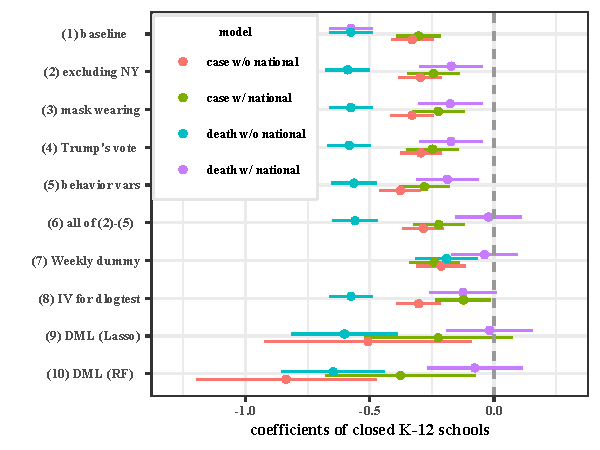
\includegraphics[width=0.5\textwidth]{tables_and_figures/pk12-whisker-7}
%          \end{tabular}
%  \end{minipage}
%    \begin{flushleft}
%      \footnotesize
%      $^\dagger$The times from exposure to case confirmation and death reporting  are assumed to be 14 and 21 days, respectively. $^\ddagger$The times from exposure to case confirmation and death reporting  are assumed to be 7 and 24 days, respectively.
%    \end{flushleft}
\end{figure}

%\begin{figure}[ht]
%  \caption{Estimated Coefficients for Mandatory Masks: Sensitivity Analysis \label{fig:whisker}}\bigskip
%    \begin{minipage}{\linewidth}
%    \centering
%      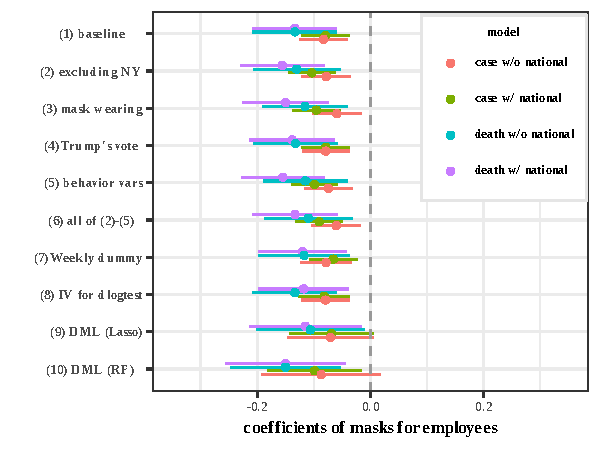
\includegraphics[width=0.5\textwidth]{tables_and_figures/pmaskbus-whisker-14}
%      \end{minipage}
%      \end{figure} 

\end{frame}

%----------------------------------------------------------------------------------------%

      %----------------------------------------------------------------------------------------% 

\begin{frame}
  \frametitle{Sensitivity Analysis: School Closures}
  
  
  \begin{figure}[ht]
%  \caption{Estimated Coefficients for  Policy Variables: Sensitivity Analysis \label{fig:whisker}}\bigskip
  \begin{minipage}{\linewidth}
    \centering
%   {\textbf{(A)  masks for employees}}\\
%    \medskip
    \begin{tabular}{cc}
 %$\quad$ School Closures &$\quad$ \\
      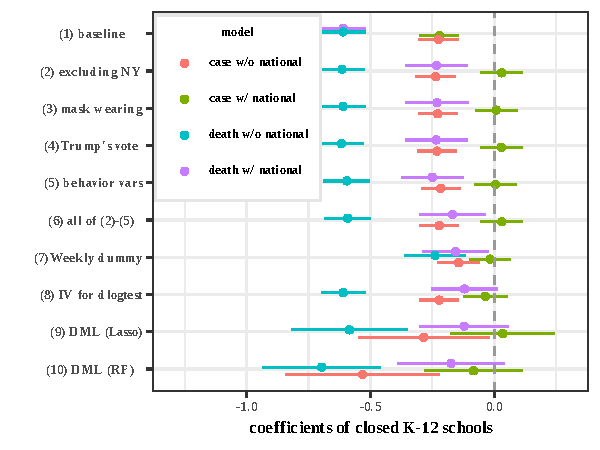
\includegraphics[width=0.49\textwidth]{tables_and_figures/pk12-whisker-14}
      &
      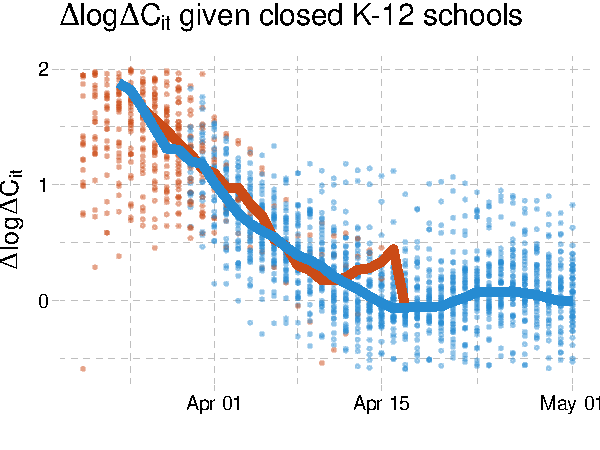
\includegraphics[width=0.49\textwidth]{tables_and_figures/pk12-cases-14}\qquad
   %        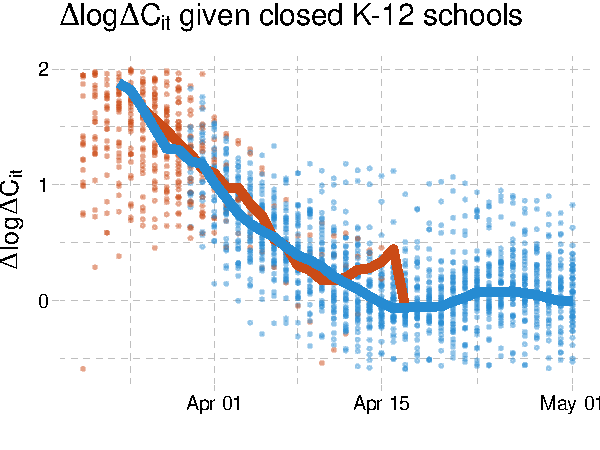
\includegraphics[width=0.483\textwidth]{tables_and_figures/pk12-cases-14}
    \end{tabular}
  \end{minipage} %\\\smallskip
%    \begin{minipage}{\linewidth}
%    \centering
%     {\textbf{(B)  closed K-12 Schools}}\\
%    \medskip
%    \begin{tabular}{cc}
% $\quad$  (i) baseline timing$^\dagger$ &$\quad$ (ii) alternative timing$^\ddagger$\\
%      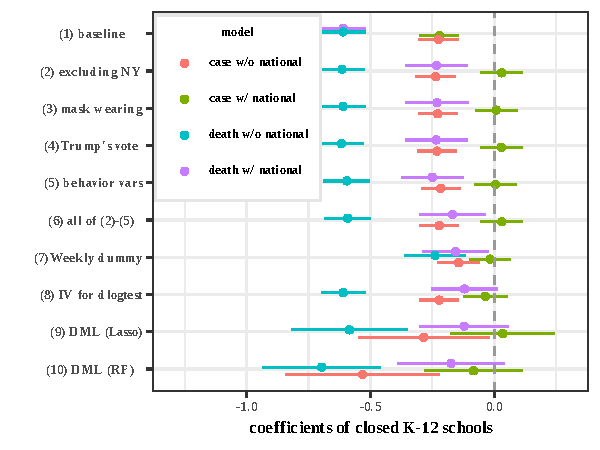
\includegraphics[width=0.5\textwidth]{tables_and_figures/pk12-whisker-14}
%      &
%      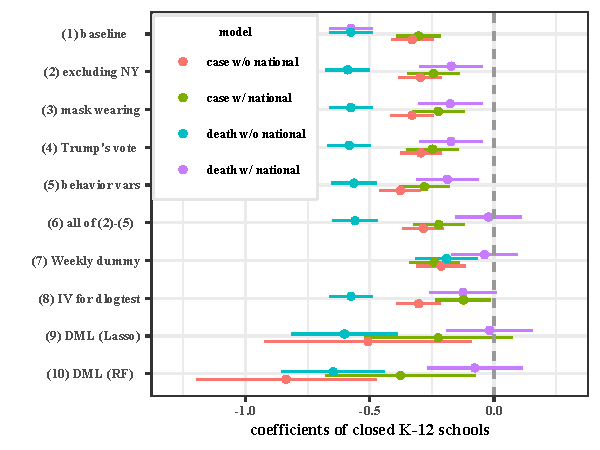
\includegraphics[width=0.5\textwidth]{tables_and_figures/pk12-whisker-7}
%          \end{tabular}
%  \end{minipage}
%    \begin{flushleft}
%      \footnotesize
%      $^\dagger$The times from exposure to case confirmation and death reporting  are assumed to be 14 and 21 days, respectively. $^\ddagger$The times from exposure to case confirmation and death reporting  are assumed to be 7 and 24 days, respectively.
%    \end{flushleft}
\end{figure}

%\begin{figure}[ht]
%  \caption{Estimated Coefficients for Mandatory Masks: Sensitivity Analysis \label{fig:whisker}}\bigskip
%    \begin{minipage}{\linewidth}
%    \centering
%      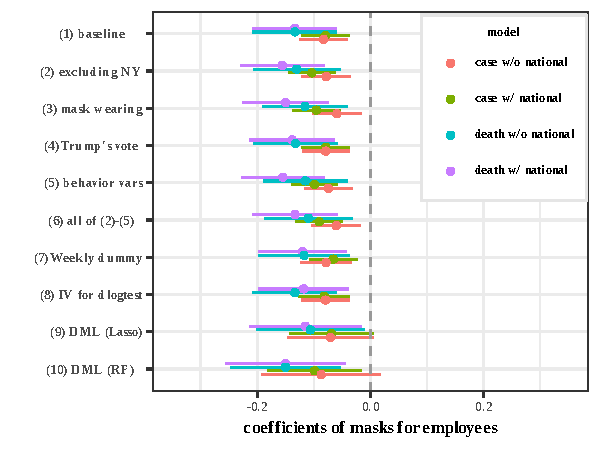
\includegraphics[width=0.5\textwidth]{tables_and_figures/pmaskbus-whisker-14}
%      \end{minipage}
%      \end{figure} 

\end{frame}

%----------------------------------------------------------------------------------------%


      %----------------------------------------------------------------------------------------% 

\begin{frame}
  \frametitle{Fixed Effects Estimator (State-level + Weekly FE)}
  \scriptsize
\begin{tabular}{@{\extracolsep{1pt}}lcc} 
\\[-1.8ex]\hline 
\hline \\[-1.8ex] 
 & \multicolumn{2}{c}{\textit{Dependent variable:}} \\ 
\cline{2-3} 
 & \multicolumn{2}{c}{$\Delta \log \Delta C_{it}$} \\ 
\\[-1.8ex] 
&FE & FE + BC\\ % & FE & FE + BC\\ 
\hline \\[-1.8ex] 
\alert{ lag(masks for employees, 14)} &\alert{ $-$0.103$^{**}$} & \alert{$-$0.271$^{***}$} \\ % & \alert{$-$0.097$^{**}$} & \alert{$-$0.255$^{***}$} \\ 
  & (0.044) & (0.075)  \\ %& (0.044) & (0.071) \\ 
  lag(closed K-12 schools, 14) & $-$0.023 & 0.085  \\ %& $-$0.050 & 0.042 \\ 
  & (0.060) & (0.098)  \\ %& (0.066) & (0.094) \\ 
  lag(stay at home, 14) & $-$0.123$^{**}$ & $-$0.088  \\ %& $-$0.099$^{**}$ & $-$0.055 \\ 
  & (0.051) & (0.068)  \\ %& (0.049) & (0.075) \\  
   lag(business closure policies, 14) & $-$0.080 & $-$0.162$^{*}$ \\ % &  &  \\ 
   & (0.076) & (0.086) \\ % &  &  \\ 
%  lag(closed movie theaters, 14) &  &  & 0.049 & 0.077 \\ 
%  &  &  & (0.068) & (0.084) \\ 
%  lag(closed restaurants, 14) &  &  & $-$0.031 & $-$0.068 \\ 
%  &  &  & (0.053) & (0.065) \\ 
%  lag(closed non-essent bus, 14) &  &  & $-$0.099$^{**}$ & $-$0.166$^{***}$ \\ 
%  &  &  & (0.047) & (0.063) \\ 
  lag($\Delta \log \Delta C_{it}$, 14) & 0.063$^{**}$ & 0.079$^{***}$ \\ % & 0.061$^{**}$ & 0.076$^{***}$ \\ 
  & (0.029) & (0.026)  \\ %& (0.029) & (0.028) \\ 
  lag($\log \Delta C_{it}$, 14) & $-$0.216$^{***}$ & $-$0.185$^{***}$ \\ % & $-$0.214$^{***}$ & $-$0.181$^{***}$ \\ 
  & (0.020) & (0.032)  \\ %& (0.021) & (0.033) \\ 
  $\Delta \log T_{it}$ & 0.116$^{***}$ & 0.116$^{***}$  \\ %& 0.118$^{***}$ \\ % & 0.147$^{***}$ \\ 
  & (0.042) & (0.042)  \\ %& (0.042) & (0.047) \\ 
 \hline \\[-1.8ex] 
Observations & 3,825 & 3,825  \\ %& 3,825 & 3,825 \\ 
R$^{2}$ & 0.782 & 0.782   \\ %& 0.782 & 0.782 \\ 
%Adjusted R$^{2}$ & 0.778 & 0.778  \\ % & 0.778 & 0.778 \\ 
\hline 
\hline \\[-1.8ex] 
%\textit{Note:}  & \multicolumn{4}{r}{$^{*}$p$<$0.1; $^{**}$p$<$0.05; $^{***}$p$<$0.01} \\ 
\end{tabular} 
  
\end{frame}

%----------------------------------------------------------------------------------------%
      
%%----------------------------------------------------------------------------------------%
%
%\begin{frame}
%  \frametitle{Discussion on Regression Results}
%  
%  
%  \begin{itemize}
%  
%   \item Death growth regression gives similar results. \smallskip
%  
%  \item The estimated effect of mandatory mask policy is robust.\smallskip
%  
%%  \item The estimated effect of stay-at-home orders is robust for cases but it is less precisely estimated for deaths.\smallskip
%  
%  \item The estimated effect of school closures is sensitive to an inclusion of national case variables. \medskip
%  
%  $\Rightarrow$ little cross-sectional variation in the timing of school closures across states.
%  
%  \end{itemize}
%  
%   
%  
%\end{frame}
%%----------------------------------------------------------------------------------------%






 


%%----------------------------------------------------------------------------------------%
%
%\begin{frame}
%  \frametitle{The Effect of Policies, Behavior, and Information on Case/Death Growth}
%
%Case Growth Regression:
%\begin{align}
% {\ycolor   \Delta \log \Delta C_{it}}
%    = {\bcolor\alpha ' B_{it}} + {\pcolor\pi 'P_{it}} + {\icolor\mu'I_{it}} + {\wcolor\delta_Y 'W_{it}}  + \varepsilon^y_{it},
% %   &  & \varepsilon^y_{it} \perp {\bcolor B_{it}}, {\pcolor P_{it}}, {\icolor I_{it}}, {\wcolor W_{it}}
%     \notag
%\end{align}
%
%Death Growth Regression:
%\begin{align}
% {\ycolor   \Delta \log \Delta D_{it}}
%    = {\bcolor\alpha ' B_{it}} + {\pcolor\pi 'P_{it}} + {\icolor\mu'I_{it}} + {\wcolor\delta_Y 'W_{it}}  + \varepsilon^y_{it},
% %   &  & \varepsilon^y_{it} \perp {\bcolor B_{it}}, {\pcolor P_{it}}, {\icolor I_{it}}, {\wcolor W_{it}}
%     \notag
%\end{align}
%
%%\begin{itemize}
%%\item ${\ycolor Y_{it}}= \Delta \log \Delta C_{it}$ or  $\Delta \log \Delta D_{it}$
%%%\item   ${\bcolor B_{it}^j}$:  ``Transit,''  ``Workplaces''  ``Grocery," and ``Retail'' \smallskip
%%%\item  $ {\pcolor  P_{it}} $ various policies \smallskip
%%%\item $ {\icolor I_{it}} $: past  cases/deaths etc. \smallskip
%%%\item $ {\wcolor   W_{it}}$: state-level characteristics   and month dummies.
%%\end{itemize}
%
%
%\end{frame}
%%----------------------------------------------------------------------------------------%



%
%
%%----------------------------------------------------------------------------------------%
%
%\begin{frame}
%  \frametitle{The Total Effect of Policies and Information on Case Growth (PI$\to$ Y)}
%
%%\textbf{Plan: will only present (1) and (3) columns for each table, possibly only for death growth}
%
%\begin{table}[!htbp] \centering
%% \caption{\label{tab:PtoY}
%%   The Total Effect of Policies on Case and Death Growth ($PI \to Y$)}\vspace{-0.3cm}
% \begin{minipage}{\linewidth}
%   \centering
%   \resizebox*{!}{\dimexpr\textheight-2\baselineskip\relax}{
%        %\resizebox{\textwidth}{!}{
%   \centering
%   \footnotesize
%\begin{tabular}{@{\extracolsep{1pt}}lcccc} 
%\\[-1.8ex]\hline 
%\hline \\[-1.8ex] 
% & \multicolumn{4}{c}{\textit{Dependent variable:}} \\ 
%\cline{2-5} 
% & \multicolumn{4}{c}{$\Delta \log \Delta C_{it}$} \\ 
%\\[-1.8ex] & (1) & (2) & (3) & (4)\\ 
%\hline \\[-1.8ex] 
%{\pcolor lag(masks for employees, 14) }& {\pcolor$-$0.081$^{**}$} &  & {\pcolor$-$0.105$^{***}$} &  \\ 
%  & (0.041) &  & (0.037) &  \\ 
%  {\pcolor lag(masks*April, 14) }&  & {\pcolor$-$0.157$^{**}$} &  &{\pcolor $-$0.146$^{**}$ }\\ 
%  &  & (0.067) &  & (0.061) \\ 
% {\pcolor lag(masks*May, 14) }&  &{\pcolor $-$0.062 }&  &{\pcolor $-$0.094$^{***}$} \\ 
%  &  & (0.039) &  & (0.036) \\ 
%  lag(closed K-12 schools, 14) & $-$0.240$^{**}$ & $-$0.241$^{**}$ & 0.009 & 0.007 \\ 
%  & (0.097) & (0.097) & (0.109) & (0.108) \\ 
%  lag(stay at home, 14) & $-$0.126$^{**}$ & $-$0.128$^{**}$ & $-$0.117$^{**}$ & $-$0.118$^{**}$ \\ 
%  & (0.055) & (0.055) & (0.052) & (0.052) \\  
% \quad\qquad $\vdots$ &$\vdots$ &$\vdots$ &$\vdots$ & $\vdots$   \\
%%  lag(closed movie theaters, 14) & 0.030 & 0.023 & 0.058 & 0.054 \\ 
%%  & (0.052) & (0.052) & (0.047) & (0.047) \\ 
%%  lag(closed restaurants, 14) & $-$0.042 & $-$0.039 & $-$0.010 & $-$0.009 \\ 
%%  & (0.049) & (0.048) & (0.045) & (0.044) \\ 
%%  lag(closed businesses, 14) & $-$0.048 & $-$0.041 & $-$0.035 & $-$0.031 \\ 
%%  & (0.050) & (0.050) & (0.044) & (0.044) \\ 
%  lag($\Delta \log \Delta C_{it}$, 14) & 0.040$^{*}$ & 0.039$^{*}$ & 0.033 & 0.032 \\ 
%  & (0.024) & (0.024) & (0.028) & (0.028) \\ 
%{\icolor lag($\log \Delta C_{it}$, 14)} &{\icolor  $-$0.138$^{***}$} &{\icolor $-$0.138$^{***}$} & {\icolor $-$0.091$^{***}$} &{\icolor  $-$0.091$^{***}$} \\ 
%  & (0.024) & (0.023) & (0.026) & (0.026) \\ 
%  lag($\Delta \log \Delta C_{it}$.national, 14) &  &  & $-$0.123$^{***}$ & $-$0.121$^{***}$ \\ 
%  &  &  & (0.043) & (0.042) \\ 
%  lag($\log \Delta C_{it}$.national, 14) &  &  & $-$0.241$^{***}$ & $-$0.239$^{***}$ \\ 
%  &  &  & (0.044) & (0.044) \\ 
%  $\Delta \log T_{it}$ & 0.157$^{***}$ & 0.158$^{***}$ & 0.161$^{***}$ & 0.161$^{***}$ \\ 
%  & (0.044) & (0.044) & (0.042) & (0.042) \\ 
% \hline \\[-1.8ex] 
%%state variables & Yes & Yes & Yes & Yes \\ 
%%Month $\times$ state variables & Yes & Yes & Yes & Yes \\ 
%%\hline \\[-1.8ex] 
%{\pcolor $\sum_j \mathrm{Policy}_j$} & {\pcolor -0.508$^{***}$} &{\pcolor  -0.644$^{***}$} &{\pcolor -0.199} & {\pcolor -0.336$^{*}$ }\\ 
% & (0.162) & (0.198) & (0.164) & (0.187) \\ 
%Observations & 3,823 & 3,823 & 3,823 & 3,823 \\ 
%%R$^{2}$ & 0.748 & 0.749 & 0.761 & 0.762 \\ 
%Adjusted R$^{2}$ & 0.746 & 0.747 & 0.759 & 0.759 \\ 
%\hline 
%\hline \\[-1.8ex] 
%%\textit{Note:}  & \multicolumn{4}{r}{$^{*}$p$<$0.1; $^{**}$p$<$0.05; $^{***}$p$<$0.01} \\ 
%\end{tabular} 
%   }
%%   \begin{flushleft}
%%     \scriptsize Dependent variable is the weekly growth rate of
%%     confirmed cases (in the left panel) or deaths (in the right
%%     panel) as defined in equation (\ref{eq:y}). The covariates
%%     include lagged policy variables, which are
%%     constructed as 7 day moving averages between $t$ to $t-7$ of
%%     corresponding daily measures.  The row
%%     ``$\sum_j \mathrm{Policies}_j$'' reports the sum of six policy
%%     coefficients.
%%   \end{flushleft}
% \end{minipage}
%   \begin{flushleft}
%\tiny
%Other policies include closures of movie theaters, restaurants, and non-essential businesses. State characteristics, month dummies, and their interactions are included.
%\end{flushleft}
%\end{table}
%
%\end{frame}
%%----------------------------------------------------------------------------------------%



%
%%----------------------------------------------------------------------------------------%
%
%\begin{frame}
%  \frametitle{Counterfactual Experiment of   Washington State   }
%
%\begin{figure}[ht]
%%  \caption{Effect of mandating masks on April 1st in Washington \label{fig:WA-mask}}
%  \begin{minipage}{\linewidth}
%    \centering
%  %%  \textbf{Fit of Case Growth Rates}\\ \bigskip
%    \begin{tabular}{cc}
% %   Washington State & Massachusetts\\
%%      \includegraphics[width=0.5\textwidth]{../tables_and_figures/Washington-mask-growth}
%%      & 
%%      \includegraphics[width=0.5\textwidth]{../tables_and_figures/Illinois-mask-growth} 
%%      
%            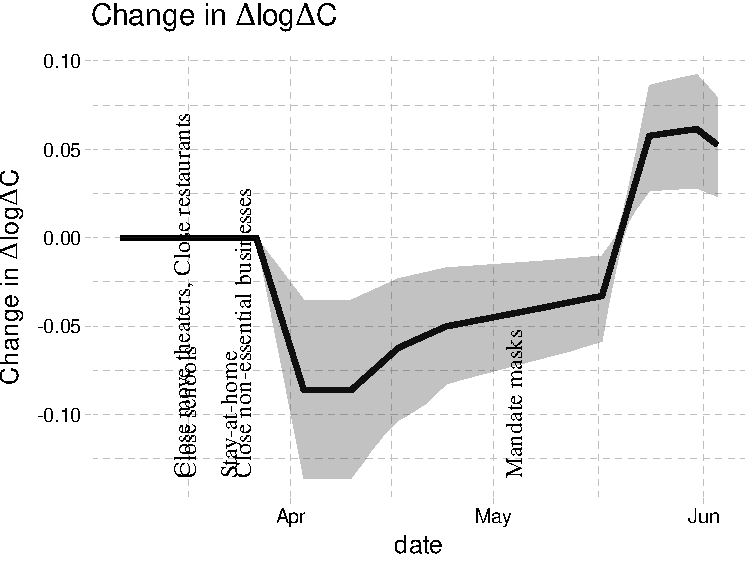
\includegraphics[width=0.5\textwidth]{tables_and_figures/Washington-mask-dgrowth_idx}
%%      &
%%        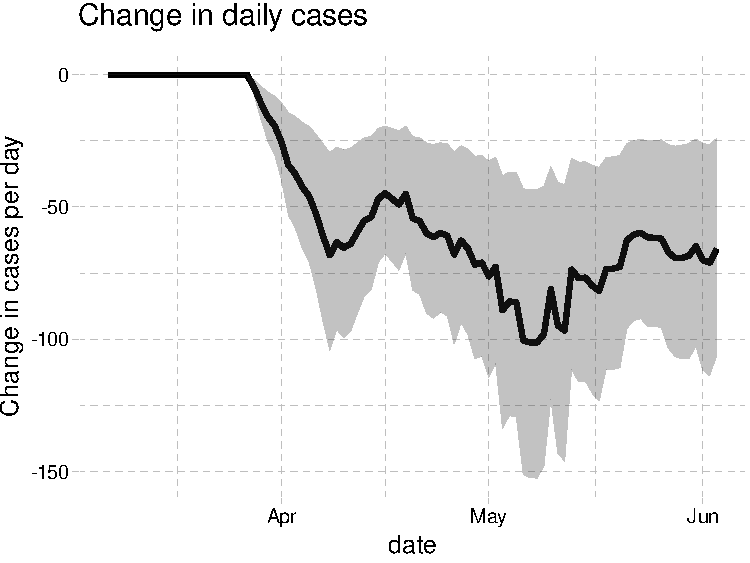
\includegraphics[width=0.31\textwidth]{tables_and_figures/Washington-mask-dcases_idx}
%      &
%        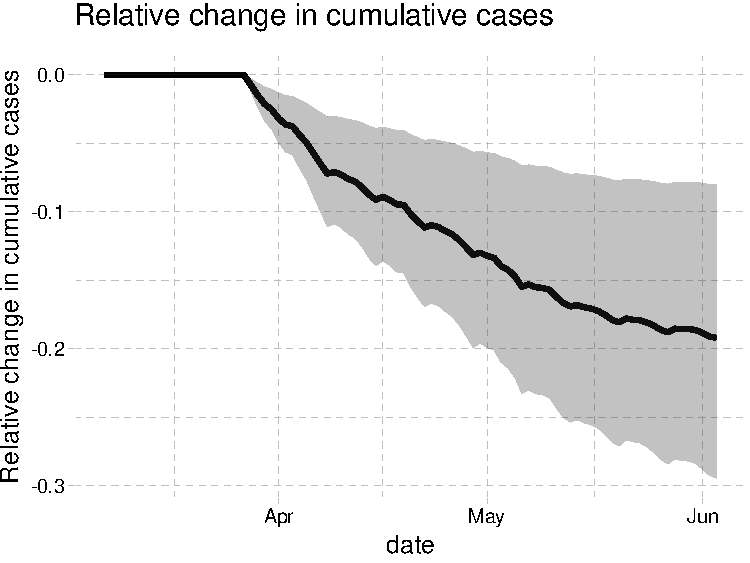
\includegraphics[width=0.5\textwidth]{tables_and_figures/Washington-mask-rcumu_idx}
%    \end{tabular}
%  \end{minipage}
%\end{figure}
%
%\end{frame}
%%----------------------------------------------------------------------------------------%


%----------------------------------------------------------------------------------------%

\begin{frame}
  \frametitle{Counterfactual Experiment of Mandating Masks on March 14th in all US states}

\vspace{-0.5cm}

\begin{figure}[ht]%\caption{Portion of states with each   policy \label{fig:policyportion}}
 % \begin{minipage}{\linewidth} 
      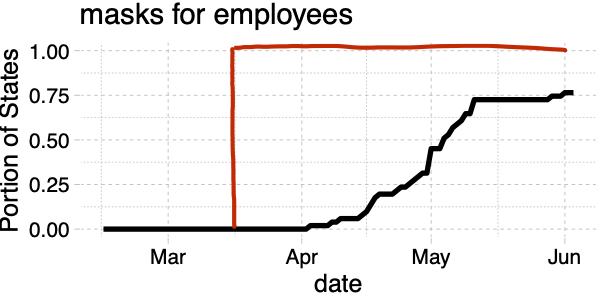
\includegraphics[width=\textwidth]{pmaskbus_p_experiment2}  
 % \end{minipage}
\end{figure}


\end{frame}
%----------------------------------------------------------------------------------------%


\begin{frame}
  \frametitle{Counterfactual Effect of Mandating Masks on March 14th in Washington State}


\begin{figure}[ht]
%  \caption{Effect of mandating masks on April 1st in Washington \label{fig:WA-mask}}
  \begin{minipage}{\linewidth}
    \centering
    \textbf{Change in Case Growth Rates}\\ \bigskip
    \begin{tabular}{c}
%      \includegraphics[width=0.5\textwidth]{../tables_and_figures/Washington-mask-growth}
%      &
      \includegraphics[width=0.8\textwidth]{../tables_and_figures/Washington-mask-dgrowth_idx}
    \end{tabular}
  \end{minipage}
\end{figure}
%\begin{figure}[ht]
%%  \caption{Effect of mandating masks on April 1st in Washington \label{fig:WA-mask}}
%  \begin{minipage}{\linewidth}
%    \centering
%    \begin{tabular}{cc}
%        \includegraphics[width=0.45\textwidth]{../tables_and_figures/Washington-mask-growth_deaths}
%      &
%        \includegraphics[width=0.45\textwidth]{../tables_and_figures/Washington-mask-dgrowth_deaths_v1}
%    \end{tabular}
%  \end{minipage}
%\end{figure}
 


\end{frame}
%----------------------------------------------------------------------------------------%

%----------------------------------------------------------------------------------------%

\begin{frame}
  \frametitle{Counterfactual Effect of Nationally Mandating Masks on March 14th in the U.S. }


\begin{figure}[ht]
%  \caption{National change in cases from mandating masks on April
%    1st\label{fig:US-mask}}
  \begin{minipage}{\linewidth}
    \centering 
    \begin{tabular}{cc}
      \textbf{Change in Case Growth} &  \textbf{Relative Decrease in Cases}\\
      \includegraphics[width=0.5\textwidth]{../tables_and_figures/us-mask-dgrowth_idx}
      &
        \includegraphics[width=0.5\textwidth]{../tables_and_figures/us-mask-rel_idx}
    \end{tabular}
  \end{minipage}
\end{figure}

%\begin{figure}[ht]
%%  \caption{National change in deaths from mandating masks on April
%%    1st\label{fig:US-mask-deaths}}
%  \begin{minipage}{\linewidth}
%    \centering
%    \begin{tabular}{cc}
%      \includegraphics[width=0.45\textwidth]{../tables_and_figures/us-mask-dgrowth_deaths_v1}
%      &
%        \includegraphics[width=0.45\textwidth]{../tables_and_figures/us-mask-rel_deaths_v1}
%    \end{tabular}
%  \end{minipage}
%\end{figure}


\end{frame}
%----------------------------------------------------------------------------------------%


%----------------------------------------------------------------------------------------%

\begin{frame}
  \frametitle{Counterfactual Effect of Nationally Mandating Masks on  March 14th in the U.S. }

%\begin{figure}[ht]
%%  \caption{National change in cases from mandating masks on April
%%    1st\label{fig:US-mask}}
%  \begin{minipage}{\linewidth}
%    \centering
%    \begin{tabular}{cc}
%      \includegraphics[width=0.45\textwidth]{../tables_and_figures/us-mask-dgrowth_v1}
%      &
%        \includegraphics[width=0.45\textwidth]{../tables_and_figures/us-mask-rel_v1}
%    \end{tabular}
%  \end{minipage}
%\end{figure}

\begin{figure}[ht]
%  \caption{National change in deaths from mandating masks on April
%    1st\label{fig:US-mask-deaths}}
  \begin{minipage}{\linewidth}
    \centering

    \begin{tabular}{cc}
      \textbf{Change in Death Growth} &  \textbf{Relative Decrease in Deaths}\\
      \includegraphics[width=0.5\textwidth]{../tables_and_figures/us-mask-dgrowth_deaths_idx}
      &
        \includegraphics[width=0.5\textwidth]{../tables_and_figures/us-mask-rel_deaths_idx}
    \end{tabular}
  \end{minipage}
\end{figure}

  19 to 47 percent less deaths nationally by the end of May
 
 $\Rightarrow$  {\ycolor 19,000 to 47,000  saved lives!!}

\end{frame}
%----------------------------------------------------------------------------------------%



%----------------------------------------------------------------------------------------%

\begin{frame}
  \frametitle{Counterfactual Experiment of No Stay-at-Home Orders in the U.S.}

\vspace{-0.5cm}
\begin{figure}[ht]%\caption{Portion of states with each   policy \label{fig:policyportion}}
  \begin{minipage}{\linewidth} 
      \includegraphics[width=\textwidth]{pshelter_p_experiment} 
  \end{minipage}
\end{figure}


\end{frame}
%----------------------------------------------------------------------------------------%



%----------------------------------------------------------------------------------------%

\begin{frame}
  \frametitle{Counterfactual Effect of No Stay-at-Home Orders in the U.S.}

 
\begin{figure}[ht]
%  \caption{Effect of having no stay-at-home orders in the US\label{fig:US-shelter}}
  \begin{minipage}{\linewidth}
    \centering
    \begin{tabular}{cc} 
      \textbf{Change in Case Growth} &  \textbf{Relative Increase in Cases}\\
      \includegraphics[width=0.5\textwidth]{../tables_and_figures/us-shelter-dgrowth_idx}
      &
        \includegraphics[width=0.5\textwidth]{../tables_and_figures/us-shelter-rel_idx}
%      \\
%      \\
%      \multicolumn{2}{c}{\textbf{Deaths}} \\
%      \includegraphics[width=0.45\textwidth]{tables_and_figures/us-shelter-dgrowth_deaths_v1}
%      &
%        \includegraphics[width=0.45\textwidth]{tables_and_figures/us-shelter-rel_deaths_v1}
    \end{tabular}
  \end{minipage}
\end{figure}

Cases would have been larger by   17 to 78 percent
 
 $\Rightarrow$  0.34 to 1.56 million more infections
 
\end{frame}
%----------------------------------------------------------------------------------------%

 
%
%%----------------------------------------------------------------------------------------%
%
%\begin{frame}
%  \frametitle{Removing all policies: Washington State}
%
%\begin{figure}[ht]
%%  \caption{Case   growth with and without policies in
%%    Washington \label{fig:WA-nop-growth}}
%  \begin{minipage}{\linewidth}
%    \centering
%    \begin{tabular}{cc}
%      \includegraphics[width=0.45\textwidth]{../tables_and_figures/Washington-nop-growth}
%      &
%        \includegraphics[width=0.45\textwidth]{../tables_and_figures/Washington-nop-dgrowth}
%    \end{tabular}
%  \end{minipage}
%\end{figure}
%
%\begin{figure}[ht]
%%  \caption{Deaths growth with and without policies in
%%    Washington \label{fig:WA-nop-growth-death}}
%  \begin{minipage}{\linewidth}
%    \centering
%    \begin{tabular}{cc}
%      \includegraphics[width=0.45\textwidth]{../tables_and_figures/Washington-nop-growth_deaths}
%      &
%        \includegraphics[width=0.45\textwidth]{../tables_and_figures/Washington-nop-dgrowth_deaths}
%    \end{tabular}
%  \end{minipage}
%\end{figure}
%
%\end{frame}
%%----------------------------------------------------------------------------------------%




%%----------------------------------------------------------------------------------------%
%
%\begin{frame}
%  \frametitle{Counterfactual Effect of Removing All Policies }
%
%
%\begin{figure}[ht]
%%  \caption{Effect of removing policies on cases: national average \label{fig:US-nop-dcases}}
%\textbf{Regression \underline{without} national case variables }
%  \begin{minipage}{\linewidth}
%    \centering
%    \begin{tabular}{cc}
%    \includegraphics[width=0.4\textwidth]{../tables_and_figures/us-nop-dgrowth_idx}
%    &
%      \includegraphics[width=0.4\textwidth]{../tables_and_figures/us-nop-rel_idx}
% %  \includegraphics[width=0.45\textwidth]{tables_and_figures/us-nop-dcases}
%      %  \includegraphics[width=0.45\textwidth]{tables_and_figures/us-nop-dgrowth_deaths}
%    \end{tabular}
%  \end{minipage}
%\end{figure} \vspace{-0.2cm}
%\begin{figure}[ht]
% % \caption{Effect of removing policies on deaths: national average \label{fig:US-nop-ddeaths}}
%\textbf{Regression \underline{with} national case variables }
%  \begin{minipage}{\linewidth}
%    \centering
%    \begin{tabular}{cc}
%      \includegraphics[width=0.4\textwidth]{../tables_and_figures/us-nop-dgrowth}
%      &
%        \includegraphics[width=0.4\textwidth]{../tables_and_figures/us-nop-rel} 
%  %  \includegraphics[width=0.45\textwidth]{tables_and_figures/us-nop-dcases_deaths}
%      %  \includegraphics[width=0.45\textwidth]{tables_and_figures/us-nop-rel}
%    \end{tabular}
%  \end{minipage}
%\end{figure}
%
%\end{frame}
%%----------------------------------------------------------------------------------------%


%----------------------------------------------------------------------------------------%

\begin{frame}
  \frametitle{Case and death growth conditional on \textbf{School Closures} }\vspace{-0.05cm}



\begin{figure}[ht]
  %\caption{Case and death growth conditional on mask mandates \label{fig:masks}}\vspace{0.2cm}
  \begin{minipage}{\linewidth}
    \centering
    \begin{tabular}{cc}
       \includegraphics[width=0.483\textwidth]{../tables_and_figures/pk12-cases}
      &
        \includegraphics[width=0.483\textwidth]{../tables_and_figures/pk12-deaths}\\
    \textbf{Case Growth} &    \textbf{Death Growth} \\  
    \end{tabular}
%    \begin{flushleft}
%      \scriptsize In these figures, red points are the case or death
%      growth rate in states without a mask mandate. Blue points are
%      states with a mask mandate 14 (21 for deaths) days prior. The
%      red line is the average across states without a mask mandate 14
%      (21 for deaths) days earlier. The blue line is the average
%      across states with a mask mandate 14 (21 for deaths) earlier.
%    \end{flushleft}
  \end{minipage}
\end{figure}

The effect of school closures is not well identified. 


\end{frame}
%----------------------------------------------------------------------------------------%


%----------------------------------------------------------------------------------------%

\begin{frame}
  \frametitle{Conclusion }

\begin{itemize}
\item  A useful framework to estimate the roles of policies and information on determining the spread of Covid-19. \smallskip
 
\item  If US-wide mask mandates had been adopted on March 14th, as much as 19,000 to 47,000 lives could have been saved by the end of May.\smallskip

\item Not having implemented Stay-at-Home Orders would have lead to  17\% to 78\% increase in cases.\smallskip

%\item Not having implemented any policy could have led to more than 7 fold increase in cases and deaths but with considerable uncertainty over the effects of school closures.
%
%


\end{itemize}
 

\end{frame}
%----------------------------------------------------------------------------------------%


%----------------------------------------------------------------------------------------%

\begin{frame}
  \frametitle{Conclusion}
  
\begin{itemize}
  
 \item Some evidence that people voluntarily reduce their mobility in response to a higher number of cases and deaths.\smallskip

 
\item There is much ambiguity related to the total effect of policies vs voluntary behavior, which can not be identified well from the US state-level data. \smallskip

\item Closure of schools has potentially large effects via behavior, keeping people at home, but school policy has almost no cross-sectional variation.\smallskip % Including national cases as information reduces the estimated school effect, resulting in greater attribution to behavior.\smallskip


%\item To Do: feedback effect from information on national cases/deaths.
  
\end{itemize}
  
\end{frame}
%----------------------------------------------------------------------------------------%

 

%----------------------------------------------------------------------------------------%

%\begin{frame}
%  \frametitle{County-level analysis}\vspace{-0.05cm}
%
%
%
%\begin{figure}[ht]
%  %\caption{Case and death growth conditional on mask mandates \label{fig:masks}}\vspace{0.2cm}
%  \begin{minipage}{\linewidth}
%    \centering 
%       \includegraphics[width=0.9\textwidth]{county-mask-cases.png} 
%%    \begin{flushleft}
%%      \scriptsize In these figures, red points are the case or death
%%      growth rate in states without a mask mandate. Blue points are
%%      states with a mask mandate 14 (21 for deaths) days prior. The
%%      red line is the average across states without a mask mandate 14
%%      (21 for deaths) days earlier. The blue line is the average
%%      across states with a mask mandate 14 (21 for deaths) earlier.
%%    \end{flushleft}
%  \end{minipage}
%\end{figure}
%
%\begin{itemize}
%\item
%Mask mandate matters!
%\item The effect of mandatory masks seems to get smaller over time, perhaps because more people voluntarily wear mask now.
%\end{itemize}
%
%\end{frame}
%%----------------------------------------------------------------------------------------% 




\begin{frame}[allowframebreaks]
\frametitle{Bibliography}
%\large
\footnotesize
\bibliography{../covid}
\end{frame}


 
\end{document}


%----------------------------------------------------------------------------------------%

\begin{frame}
  \frametitle{Direct and Indirect Policy Effects for Death Regression}

\begin{table}
 % \caption{\label{tab:dieff}Direct and Indirect Policy Effects}
\begin{minipage}{\linewidth}
  \centering
    \tiny
  \begin{tabular}{c}
%    \textbf{Cases}
%    \\
%    \input{tables_and_figures/dieff-cases}
      \\
    \textbf{{\normalsize Death Growth Regression  \underline{without national death variables}}}
    \\
    \\
\begin{tabular}{lccc|c|c|c}
\toprule
&\multicolumn{3}{c|}{ PI$\to$B Coef.\ \& \ PBI$\to$Y Coef.  } &PI$\to$Y Coef.  & Average & Difference \\
  & Direct & Indirect & Total & Total  & Total &(over-id test)  \\\
  &${\pcolor\pi'}$&${\bcolor\alpha '}  {\pcolor \beta' }$ &${\pcolor\pi'}+{\bcolor\alpha '}  {\pcolor \beta' }$ &${\pcolor\pi'}+{\bcolor\alpha '}  {\pcolor \beta' }$ &${\pcolor\pi'}+{\bcolor\alpha '}  {\pcolor \beta' }$  & \\
\midrule
Mask for Employees & \alert{  -0.145$^{***}$} & \alert{  -0.004} &  \alert{ -0.149$^{***}$} & \alert{  -0.133$^{***}$} &  \alert{ -0.141$^{***}$} & \alert{  -0.016}\\
 & (0.050) & (0.023) & (0.055) & (0.051) & (0.052) & (0.015)\\
School Closures & -0.271$^{***}$ & -0.451$^{***}$ & -0.722$^{***}$ & -0.641$^{***}$ & -0.681$^{***}$ & -0.081$^{***}$\\
 & (0.092) & (0.082) & (0.111) & (0.107) & (0.108) & (0.026)\\
Stay-at-Home & -0.040 & -0.034 & -0.074 & -0.080 & -0.077 & 0.006\\
 & (0.064) & (0.035) & (0.064) & (0.064) & (0.064) & (0.015)\\ 
 \quad\qquad $\vdots$ &$\vdots$ &$\vdots$ &$\vdots$ &$\vdots$ &$\vdots$ &$\vdots$  \\\hline
%closed movie theaters & 0.039 & -0.025 & 0.014 & 0.018 & 0.016 & -0.004\\
% & (0.091) & (0.030) & (0.089) & (0.089) & (0.088) & (0.018)\\
%closed restaurants & 0.085 & -0.105$^{**}$ & -0.020 & -0.015 & -0.018 & -0.005\\
% & (0.065) & (0.042) & (0.056) & (0.057) & (0.056) & (0.016)\\
%closed businesses & -0.003 & -0.024 & -0.027 & -0.038 & -0.032 & 0.011\\
% & (0.055) & (0.021) & (0.061) & (0.063) & (0.062) & (0.013)\\
$\sum_j \mathrm{Policy}_j$ & -0.334$^{**}$ & -0.644$^{***}$ & -0.979$^{***}$ & -0.889$^{***}$ & -0.934$^{***}$ & -0.090$^{**}$\\
 & (0.160) & (0.154) & (0.171) & (0.165) & (0.167) & (0.035)\\
%$\Delta \log \Delta D_{it}$ & 0.016 & -0.025$^{**}$ & -0.009 & -0.000 & -0.004 & -0.009$^{*}$\\
% & (0.034) & (0.011) & (0.031) & (0.032) & (0.031) & (0.005)\\
%$\log \Delta D_{it}$ & -0.051$^{**}$ & -0.018$^{*}$ & -0.069$^{**}$ & -0.078$^{***}$ & -0.073$^{***}$ & 0.009$^{*}$\\
% & (0.024) & (0.010) & (0.028) & (0.026) & (0.027) & (0.005)\\
\bottomrule
\end{tabular}
    \\
  \end{tabular}
%  \smallskip
%  \begin{flushleft}
%      \scriptsize Direct effects capture the effect of policy on case
%      growth holding behavior, information, and confounders
%      constant. Direct effects are given by ${\pcolor \pi}$ in
%      equation (\ref{eq:R1}). Indirect effects capture how policy
%      changes behavior and behavior shift case growth. They are given
%      by ${\bcolor \alpha}$ from (\ref{eq:R1}) times ${\pcolor \beta}$
%      from (\ref{eq:R2}). The total effect is
%      ${\pcolor \pi} + {\pcolor \beta} {\bcolor \alpha}$. Column
%      ``PI$\to$Y Coefficients'' shows the coefficient estimates from
%      \ref{eq:R4}. Columns ``Difference''    are  the differences between
%      the estimates from (\ref{eq:R4}) and the combination of
%      (\ref{eq:R1}) and (\ref{eq:R2}) while column ``Average'' are their averages.
%      Standard errors are computed by
%      bootstrap and clustered on state.
%    %  \ref{tab:PtoY}.
%    \end{flushleft}
  \end{minipage}
\end{table}
\begin{flushleft}
\footnotesize
Other policies include closures of movie theaters, restaurants, and non-essential businesses.
\end{flushleft}
\end{frame}
%----------------------------------------------------------------------------------------%



%----------------------------------------------------------------------------------------%

\begin{frame}
  \frametitle{Direct and Indirect Policy Effects for Death Regression}

\begin{table}
 % \caption{\label{tab:dieff}Direct and Indirect Policy Effects}
\begin{minipage}{\linewidth}
  \centering
    \tiny
  \begin{tabular}{c}
%    \textbf{Cases}
%    \\
%    \input{tables_and_figures/dieff-cases}
      \\
    \textbf{{\normalsize Death Growth Regression  \underline{with national death variables}}}
    \\
    \\
\begin{tabular}{lccc|c|c|c}
\toprule
&\multicolumn{3}{c|}{ PI$\to$B Coef.\ \& \ PBI$\to$Y Coef.  } &PI$\to$Y Coef. & Average & Difference \\
  & Direct & Indirect & Total & Total  & Total & (over-id test) \\\
  &${\pcolor\pi'}$&${\bcolor\alpha '}  {\pcolor \beta' }$ &${\pcolor\pi'}+{\bcolor\alpha '}  {\pcolor \beta' }$ &${\pcolor\pi'}+{\bcolor\alpha '}  {\pcolor \beta' }$ & & \\
\midrule
Masks for Employees & \alert{ -0.148$^{***}$} &\alert{ -0.018} & \alert{-0.166$^{***}$} &\alert{ -0.161$^{***}$} &\alert{ -0.164$^{***}$} &\alert{ -0.005}\\
 & (0.048) & (0.023) & (0.053) & (0.050) & (0.051) & (0.016)\\
School Closures & -0.199$^{**}$ & -0.038 & -0.238$^{**}$ & -0.250$^{**}$ & -0.244$^{**}$ & 0.012\\
 & (0.091) & (0.038) & (0.100) & (0.099) & (0.099) & (0.020)\\
Stay-at-Home  & -0.047 & -0.030 & -0.077 & -0.075 & -0.076 & -0.002\\
 & (0.065) & (0.032) & (0.063) & (0.063) & (0.063) & (0.014)\\ 
 \quad\qquad $\vdots$ &$\vdots$ &$\vdots$ &$\vdots$ &$\vdots$ &$\vdots$ &$\vdots$  \\\hline
%closed movie theaters & 0.054 & 0.007 & 0.061 & 0.065 & 0.063 & -0.004\\
% & (0.090) & (0.021) & (0.086) & (0.083) & (0.084) & (0.016)\\
%closed restaurants & 0.081 & -0.058$^{**}$ & 0.023 & 0.031 & 0.027 & -0.008\\
% & (0.064) & (0.024) & (0.053) & (0.054) & (0.053) & (0.014)\\
%closed businesses & -0.003 & 0.003 & -0.000 & -0.012 & -0.006 & 0.012\\
% & (0.056) & (0.016) & (0.059) & (0.060) & (0.059) & (0.012)\\
$\sum_j \mathrm{Policy}_j$ & -0.262 & -0.135 & -0.397$^{**}$ & -0.402$^{**}$ & -0.399$^{**}$ & 0.005\\
 & (0.167) & (0.085) & (0.179) & (0.174) & (0.176) & (0.024)\\
%$\Delta \log \Delta D_{it}$ & 0.017 & -0.002 & 0.015 & 0.019 & 0.017 & -0.004\\
% & (0.037) & (0.005) & (0.036) & (0.036) & (0.036) & (0.004)\\
%$\log \Delta D_{it}$ & -0.049$^{**}$ & -0.006 & -0.055$^{**}$ & -0.062$^{**}$ & -0.059$^{**}$ & 0.007\\
% & (0.024) & (0.009) & (0.028) & (0.027) & (0.027) & (0.005)\\
%$\Delta \log \Delta D_{it}$.national & -0.046 & -0.069$^{***}$ & -0.115$^{**}$ & -0.160$^{***}$ & -0.137$^{***}$ & 0.045$^{***}$\\
% & (0.046) & (0.021) & (0.050) & (0.057) & (0.053) & (0.013)\\
%$\log \Delta D_{it}$.national & -0.060 & -0.097$^{***}$ & -0.157$^{***}$ & -0.120$^{***}$ & -0.138$^{***}$ & -0.037$^{***}$\\
 & (0.038) & (0.029) & (0.032) & (0.029) & (0.030) & (0.012)\\
\bottomrule
\end{tabular}
    \\
  \end{tabular}
%  \smallskip
%  \begin{flushleft}
%      \scriptsize Direct effects capture the effect of policy on case
%      growth holding behavior, information, and confounders
%      constant. Direct effects are given by ${\pcolor \pi}$ in
%      equation (\ref{eq:R1}). Indirect effects capture how policy
%      changes behavior and behavior shift case growth. They are given
%      by ${\bcolor \alpha}$ from (\ref{eq:R1}) times ${\pcolor \beta}$
%      from (\ref{eq:R2}). The total effect is
%      ${\pcolor \pi} + {\pcolor \beta} {\bcolor \alpha}$. Column
%      ``PI$\to$Y Coefficients'' shows the coefficient estimates from
%      \ref{eq:R4}. Columns ``Difference''    are  the differences between
%      the estimates from (\ref{eq:R4}) and the combination of
%      (\ref{eq:R1}) and (\ref{eq:R2}) while column ``Average'' are their averages.
%      Standard errors are computed by
%      bootstrap and clustered on state.
%    %  \ref{tab:PtoY}.
%    \end{flushleft}
  \end{minipage}
\end{table}
\begin{flushleft}
\footnotesize
Other policies include closures of movie theaters, restaurants, and non-essential businesses.
\end{flushleft}
\end{frame}
%----------------------------------------------------------------------------------------%

%----------------------------------------------------------------------------------------%

\begin{frame}
  \frametitle{Counterfactual Experiments}

\begin{itemize}
\item
Set initial \(\Delta \log \Delta D\) and
\(\log \Delta D\)  to their first observed values. \smallskip
\item  Other regressors at their observed
values. \smallskip
\item Error terms are drawn with replacement from the residuals.\smallskip
\item Do this many times and report the average over draws of the
residuals to obtain counterfactual results.   \smallskip

\item To obtain a point-wise 90\% confidence interval, we repeat the above with
coefficients drawn randomly from their asymptotic distribution.

 
\end{itemize}


\end{frame}
%----------------------------------------------------------------------------------------%


%----------------------------------------------------------------------------------------%

\begin{frame}
  \frametitle{The Effect of Policies and Information on Behavior (PI$\to$ B)}

  % \textbf{Plan: will only present (5)-(8) columns}
  % behavior-deathsinfo-nationinfo-pib is columns (5)-(8)
  % behavior-deathsinfo-stateinfo-pib is columns (1)-(4)
  % for cases:
  % behavior-cases-nationinfo-pib is columns (5)-(8)
  % behavior-cases-stateinfo-pib is columns (1)-(4)
  
  
\begin{table}[!htbp] \centering
% \caption{The Direct Effect of Behavior and Policies on Case and
%   Death Growth ($PBI \to Y$)}\vspace{-0.3cm}
 \begin{minipage}{\linewidth}
   \centering 
   Cases as Information
   \resizebox*{!}{\dimexpr\textheight-2\baselineskip\relax}{ 
     \tiny       \begin{tabular}{@{\extracolsep{1pt}}lcccccccc} 
\\[-1.8ex]\hline 
\hline \\[-1.8ex] 
 & \multicolumn{8}{c}{\textit{Dependent variable:}} \\ 
\cline{2-9} 
 & Workplaces & Retail & Grocery &   Transit & Workplaces & Retail & Grocery &    Transit \\ 
\\[-1.8ex] & (1) & (2) & (3) & (4) & (5) & (6) & (7) &(8)  \\ 
\hline \\[-1.8ex]  
 masks for employees & $-$0.011 & $-$1.207 & $-$2.178$^{**}$ & $-$3.104 & $-$0.812 & $-$2.422$^{*}$ & $-$2.422$^{***}$ & $-$4.044$^{*}$ \\ 
  & (0.873) & (1.513) & (0.952) & (2.213) & (0.660) & (1.347) & (0.902) & (2.094) \\ 
  closed K-12 schools & $-$19.678$^{***}$ & $-$21.898$^{***}$ & $-$13.021$^{***}$ & $-$22.694$^{***}$ & $-$4.908$^{***}$ & $-$1.873 & $-$7.923$^{***}$ & $-$5.147 \\ 
  & (2.830) & (4.409) & (2.536) & (5.597) & (1.526) & (1.979) & (2.944) & (4.868) \\ 
  stay at home & $-$2.943$^{***}$ & $-$5.625$^{***}$ & $-$5.598$^{***}$ & $-$8.577$^{***}$ & $-$3.222$^{***}$ & $-$6.306$^{***}$ & $-$5.620$^{***}$ & $-$8.881$^{***}$ \\ 
  & (1.045) & (1.346) & (1.361) & (2.366) & (0.957) & (1.154) & (1.356) & (2.347) \\ 
  closed movie theaters & $-$1.975$^{*}$ & $-$3.444$^{**}$ & $-$2.897$^{**}$ & 1.129 & $-$1.464$^{*}$ & $-$3.061$^{**}$ & $-$2.643$^{**}$ & 1.764 \\ 
  & (1.103) & (1.607) & (1.200) & (2.359) & (0.820) & (1.310) & (1.150) & (2.252) \\ 
  closed restaurants & $-$3.151$^{***}$ & $-$7.682$^{***}$ & $-$1.431$^{*}$ & $-$7.969$^{***}$ & $-$1.435$^{**}$ & $-$5.095$^{***}$ & $-$0.903 & $-$5.954$^{**}$ \\ 
  & (1.012) & (1.500) & (0.756) & (2.557) & (0.698) & (1.002) & (0.623) & (2.365) \\ 
  closed businesses & $-$1.942$^{*}$ & $-$1.742 & $-$2.390$^{**}$ & $-$1.300 & $-$2.131$^{**}$ & $-$2.147$^{*}$ & $-$2.418$^{**}$ & $-$1.510 \\ 
  & (1.116) & (1.362) & (1.044) & (2.039) & (0.908) & (1.125) & (0.981) & (1.917) \\ 
  $\Delta \log \Delta C_{it}$ & 1.791$^{***}$ & 1.046$^{**}$ & 1.870$^{***}$ & 1.857$^{***}$ & 1.596$^{***}$ & 1.155$^{***}$ & 1.710$^{***}$ & 1.591$^{***}$ \\ 
  & (0.356) & (0.532) & (0.376) & (0.553) & (0.221) & (0.378) & (0.403) & (0.601) \\ 
  $\log \Delta C_{it}$ & $-$2.107$^{***}$ & $-$1.934$^{**}$ & 0.225 & $-$1.092 & $-$0.366 & 0.210 & 0.880 & 0.997 \\ 
  & (0.493) & (0.900) & (0.481) & (1.175) & (0.340) & (0.784) & (0.542) & (1.285) \\ 
  $\Delta \log \Delta C_{it}$.national &  &  &  &  & $-$2.998$^{***}$ & $-$6.952$^{***}$ & $-$0.319 & $-$3.294$^{***}$ \\ 
  &  &  &  &  & (0.452) & (0.759) & (0.680) & (1.187) \\ 
  $\log \Delta C_{it}$.national &  &  &  &  & $-$6.610$^{***}$ & $-$8.957$^{***}$ & $-$2.283$^{***}$ & $-$7.854$^{***}$ \\ 
  &  &  &  &  & (0.440) & (0.853) & (0.826) & (1.396) \\ 
 \hline \\[-1.8ex] 
state variables & Yes & Yes & Yes & Yes & Yes & Yes & Yes & Yes \\ 
Month $\times$ state variables & Yes & Yes & Yes & Yes & Yes & Yes & Yes & Yes \\ 
\hline \\[-1.8ex] 
$\sum_j \mathrm{Policy}_j$ & -29.699$^{***}$ & -41.597$^{***}$ & -27.515$^{***}$ & -42.515$^{***}$ & -13.972$^{***}$ & -20.904$^{***}$ & -21.931$^{***}$ & -23.772$^{***}$ \\ 
 & (3.296) & (5.343) & (3.246) & (6.813) & (1.953) & (2.859) & (3.325) & (5.127) \\ 
Observations & 4,284 & 4,284 & 4,284 & 4,284 & 4,284 & 4,284 & 4,284 & 4,284 \\ 
R$^{2}$ & 0.912 & 0.854 & 0.788 & 0.812 & 0.945 & 0.902 & 0.794 & 0.836 \\ 
Adjusted R$^{2}$ & 0.912 & 0.853 & 0.786 & 0.810 & 0.945 & 0.901 & 0.793 & 0.835 \\ 
\hline 
\end{tabular}  }
% \begin{flushleft}
%     \scriptsize Dependent variable is the weekly growth rate of
%     confirmed cases (in the left panel) or deaths (in the right
%     panel) as defined in equation (\ref{eq:y}). The covariates
%     include lagged policy and behavior variables, which are
%     constructed as 7 day moving averages between $t$ to $t-7$ of
%     corresponding daily measures.  The row
%     ``$\sum_j \mathrm{Policies}_j$'' reports the sum of six policy
%     coefficients.  The row ``$\sum_k w_k \mathrm{Behavior}_k$''
%     reports the sum of four coefficients of behavior variables
%     weighted by the average of each behavioral variable from April
%     1st-10th.
%   \end{flushleft}
 \end{minipage} \vspace{-0.4cm}
  \begin{flushleft}
\tiny
%Other policies include closures of movie theaters, restaurants, and non-essential businesses. State characteristics, month dummies, and their interactions are included.
\end{flushleft}
\end{table}

 
\end{frame}
%----------------------------------------------------------------------------------------%


%----------------------------------------------------------------------------------------%

\begin{frame}
  \frametitle{The Effect of Policies and Information on Behavior (PI$\to$ B)}

  % \textbf{Plan: will only present (5)-(8) columns}
  % behavior-deathsinfo-nationinfo-pib is columns (5)-(8)
  % behavior-deathsinfo-stateinfo-pib is columns (1)-(4)
  % for cases:
  % behavior-cases-nationinfo-pib is columns (5)-(8)
  % behavior-cases-stateinfo-pib is columns (1)-(4)
  
  
\begin{table}[!htbp] \centering
% \caption{The Direct Effect of Behavior and Policies on Case and
%   Death Growth ($PBI \to Y$)}\vspace{-0.3cm}
 \begin{minipage}{\linewidth}
   \centering
    Deaths as Information
   \resizebox*{!}{\dimexpr\textheight-2\baselineskip\relax}{
     \tiny       \begin{tabular}{@{\extracolsep{1pt}}lcccccccc} 
\\[-1.8ex]\hline 
\hline \\[-1.8ex] 
 & \multicolumn{8}{c}{\textit{Dependent variable:}} \\ 
\cline{2-9} 
 & Workplaces & Retail & Grocery &   Transit & Workplaces & Retail & Grocery &    Transit \\ 
\\[-1.8ex] & (1) & (2) & (3) & (4) & (5) & (6) & (7) &(8)  \\ 
\hline \\[-1.8ex]  
  masks for employees & $-$0.477 & $-$2.217 & $-$2.720$^{**}$ & $-$3.914$^{*}$ & $-$1.335$^{**}$ & $-$3.487$^{**}$ & $-$3.156$^{***}$ & $-$4.857$^{**}$ \\ 
  & (0.753) & (1.415) & (1.059) & (2.320) & (0.642) & (1.389) & (0.989) & (2.270) \\ 
  closed K-12 schools & $-$24.156$^{***}$ & $-$26.171$^{***}$ & $-$12.250$^{***}$ & $-$24.946$^{***}$ & $-$5.355$^{***}$ & $-$1.900 & $-$3.859 & $-$5.245 \\ 
  & (2.253) & (3.220) & (1.771) & (3.818) & (1.703) & (1.934) & (2.378) & (4.737) \\ 
  stay at home & $-$2.579$^{***}$ & $-$5.589$^{***}$ & $-$6.090$^{***}$ & $-$8.761$^{***}$ & $-$2.799$^{***}$ & $-$5.998$^{***}$ & $-$6.229$^{***}$ & $-$9.024$^{***}$ \\ 
  & (0.985) & (1.347) & (1.523) & (2.513) & (0.959) & (1.188) & (1.518) & (2.557) \\ 
  closed movie theaters & $-$2.298$^{**}$ & $-$4.148$^{**}$ & $-$3.102$^{**}$ & 0.658 & $-$1.032 & $-$2.661$^{*}$ & $-$2.585$^{**}$ & 1.945 \\ 
  & (1.140) & (1.693) & (1.229) & (2.364) & (0.820) & (1.379) & (1.144) & (2.321) \\ 
  closed restaurants & $-$3.479$^{***}$ & $-$7.579$^{***}$ & $-$1.317$^{*}$ & $-$7.934$^{***}$ & $-$1.507$^{**}$ & $-$4.919$^{***}$ & $-$0.400 & $-$5.838$^{**}$ \\ 
  & (1.104) & (1.559) & (0.752) & (2.583) & (0.707) & (1.016) & (0.660) & (2.437) \\ 
  closed businesses & $-$2.106$^{**}$ & $-$2.351$^{*}$ & $-$2.516$^{**}$ & $-$1.656 & $-$1.072 & $-$0.977 & $-$2.042$^{*}$ & $-$0.563 \\ 
  & (1.055) & (1.343) & (1.126) & (2.077) & (0.896) & (1.160) & (1.050) & (2.023) \\ 
  $\Delta \log \Delta D_{it}$ & $-$0.922$^{**}$ & $-$2.050$^{***}$ & $-$0.469 & $-$1.263$^{**}$ & 0.115 & $-$0.278 & 0.136 & $-$0.061 \\ 
  & (0.407) & (0.595) & (0.418) & (0.619) & (0.237) & (0.438) & (0.422) & (0.578) \\ 
  $\log \Delta D_{it}$ & $-$1.077$^{***}$ & $-$0.185 & 0.057 & $-$0.262 & $-$0.644 & 0.155 & 0.179 & 0.134 \\ 
  & (0.389) & (0.741) & (0.565) & (1.195) & (0.409) & (0.790) & (0.609) & (1.284) \\ 
  $\Delta \log \Delta D_{it}$.national &  &  &  &  & $-$4.066$^{***}$ & $-$6.883$^{***}$ & $-$2.351$^{***}$ & $-$4.695$^{***}$ \\ 
  &  &  &  &  & (0.353) & (0.619) & (0.449) & (0.833) \\ 
  $\log \Delta D_{it}$.national &  &  &  &  & $-$6.322$^{***}$ & $-$7.884$^{***}$ & $-$2.731$^{***}$ & $-$6.551$^{***}$ \\ 
  &  &  &  &  & (0.420) & (0.594) & (0.561) & (0.997) \\ 
 \hline \\[-1.8ex] 
state variables & Yes & Yes & Yes & Yes & Yes & Yes & Yes & Yes \\ 
Month $\times$ state variables & Yes & Yes & Yes & Yes & Yes & Yes & Yes & Yes \\ 
\hline \\[-1.8ex] 
$\sum_j \mathrm{Policy}_j$ & -35.094$^{***}$ & -48.055$^{***}$ & -27.995$^{***}$ & -46.554$^{***}$ & -13.100$^{***}$ & -19.941$^{***}$ & -18.270$^{***}$ & -23.581$^{***}$ \\ 
 & (2.253) & (3.604) & (2.982) & (5.781) & (2.119) & (3.144) & (3.258) & (6.007) \\ 
Observations & 4,284 & 4,284 & 4,284 & 4,284 & 4,284 & 4,284 & 4,284 & 4,284 \\ 
R$^{2}$ & 0.902 & 0.850 & 0.778 & 0.810 & 0.943 & 0.905 & 0.792 & 0.834 \\ 
Adjusted R$^{2}$ & 0.902 & 0.849 & 0.776 & 0.809 & 0.943 & 0.904 & 0.791 & 0.833 \\ 
\hline 
\end{tabular}  }
% \begin{flushleft}
%     \scriptsize Dependent variable is the weekly growth rate of
%     confirmed cases (in the left panel) or deaths (in the right
%     panel) as defined in equation (\ref{eq:y}). The covariates
%     include lagged policy and behavior variables, which are
%     constructed as 7 day moving averages between $t$ to $t-7$ of
%     corresponding daily measures.  The row
%     ``$\sum_j \mathrm{Policies}_j$'' reports the sum of six policy
%     coefficients.  The row ``$\sum_k w_k \mathrm{Behavior}_k$''
%     reports the sum of four coefficients of behavior variables
%     weighted by the average of each behavioral variable from April
%     1st-10th.
%   \end{flushleft}
 \end{minipage} \vspace{-0.4cm}
  \begin{flushleft}
\tiny
%Other policies include closures of movie theaters, restaurants, and non-essential businesses. State characteristics, month dummies, and their interactions are included.
\end{flushleft}
\end{table}

 
\end{frame}
%----------------------------------------------------------------------------------------%





\begin{frame}[allowframebreaks]
\frametitle{Bibliography}
%\large
\footnotesize
\bibliography{../covid}
\end{frame}

 
\end{document}
 



%----------------------------------------------------------------------------------------%

\begin{frame}
  \frametitle{The Effect of Policies and Information on Behavior}

% We first examine how policies and information affect social distancing behaviors by estimating a version of (\ref{eq:R2}):
\begin{align}
  {\bcolor B_{it}^j}
  %& = {\pcolor (\beta^j)' P_{it} }  + {\icolor \gamma_{1}^j \log(t) + \gamma_{2}^j \log (\Delta C_{i,t-14}) +  \gamma_{3}^j Y_{i,t-7}} + {\wcolor (\delta_B^j)' W_{it}} + \varepsilon_{it}^j \nonumber\\
  & = {\pcolor (\beta^j)' P_{it}} + {\icolor (\gamma^j)' I_{it}} +
    {\wcolor (\delta_B^j)' W_{it}} + \varepsilon_{it}^{bj}, \notag
\end{align}

\begin{itemize}
\item   ${\bcolor B_{it}^j}$:  ``Transit,''  ``Workplaces''  ``Grocery," and ``Retail'' from Google Mobility Reports,\smallskip
\item  $ {\pcolor  P_{it}} $: masks for employees, stay at home, closure of schools, closure of movie theaters, closure of non-essential businesses.\smallskip
\item $ {\icolor I_{it}} $: past growth of cases/deaths, the log of past cases/deaths, national-level cases/deaths and their growth.\smallskip
\item $ {\wcolor   W_{it}}$: state-level characteristics   and month dummies.
 
%----------------------------------------------------------------------------------------%

\begin{frame}
  \frametitle{Counterfactual Experiments}

\begin{itemize}
\item
Set initial \(\Delta \log \Delta D\) and
\(\log \Delta D\)  to their first observed values. \smallskip
\item  Other regressors at their observed
values. \smallskip
\item Error terms are drawn with replacement from the residuals.\smallskip
\item Do this many times and report the average over draws of the
residuals to obtain counterfactual results.   \smallskip

\item To obtain a point-wise 90\% confidence interval, we repeat the above with
coefficients drawn randomly from their asymptotic distribution.

 
\end{itemize}


\end{frame}
%----------------------------------------------------------------------------------------%

 

\begin{frame}[allowframebreaks]
\frametitle{Bibliography}
%\large
\footnotesize
\bibliography{covid}
%\bibliography{../covid}
\end{frame}


 
\end{document}

  
=======
%----------------------------------------------------------------------------------------%

\begin{frame}
  \frametitle{SIR Model and Empirical Specification}\vspace{-0.05cm}

 SIR Model with confirmed cases $ \dot{C}(t)$ and testing $\tau(t)$:
\begin{align*}
  \dot{S}(t)  = -\frac{S(t)}{N} \beta(t) \Infected(t),\qquad
 & \dot{\Infected}(t)   = \frac{S(t)}{N} \beta(t) \Infected(t) - \gamma  \Infected(t), \\
  % \frac{S(t-\ell)}{N} \beta(t-\ell)  \Infected(t-\ell) \label{eq:i} \\
  \dot{\Recovered}(t)   = (1-\kappa) \gamma  \Infected(t),\qquad %  \frac{S(t-\ell)}{N} \beta(t-\ell)    \Infected(t-\ell) \label{eq:r} \\
 &  \dot{D}(t) = \kappa \gamma \Infected(t), %  \frac{S(t-\ell)}{N} \beta(t-\ell)   \Infected(t-\ell)
\qquad \dot{C}(t) = \tau(t) \Infected(t). \qquad
\end{align*}


  Differentiating  { $\dot{C}(t) = \tau(t) \Infected(t)$},
  \begin{align*}
    \frac{\ddot{C}(t)}{\dot{C}(t)}
              & =
                \frac{S(t)}{N} \beta(t) -\gamma  + \frac{\dot{\tau}(t)}{\tau(t)}.
                \end{align*}
       Discrete-time analogue with $\frac{S(t)}{N} \beta(t)\approx  X_{it}' \theta + \epsilon_{it}$:\medskip
   \begin{align*}
 {\ycolor Y_{it} }:=   {\ycolor \Delta \log \Delta C_{it}}    = X_{it}' \theta + \epsilon_{it} - \gamma+\delta_T {\wcolor \Delta
      \log(T)_{it}}.
                 \end{align*}



\end{frame}

%----------------------------------------------------------------------------------------%


\end{document}
	
>>>>>>> counterfactuals
